\section{Meshes and wall neighborhoods}
\label{sec:mesh}

This section constructs wall neighborhoods satisfying the geometric
hypotheses of Definition~\ref{wl:prestack}, with fixed-factor bounds
for their scalar parameter slopes.  Section~\ref{sec:calibrated-islands}
will improve those bounds on the calibrated source patches.
The analytic selection of the edge tests and the
guard-independent integral capacities is made in
Lemma~\ref{ha:ambient-tests} and Lemma~\ref{ha:capacities};
Proposition~\ref{ha:initial-walls} transfers their counts to the actual
starting walls.  We separate those
selections from the geometric estimates: all statements below concerning
an edge count are conditional on that count, and their constants do not
depend on the final sample weights or on the mesh resolution.

Two different estimates are needed.  Away from the calibrated source
patches, a fixed multiple of the weighted edge counts suffices to bound
the scalar parameter slopes.  On those finitely many patches, the
later gradient argument requires nearly sharp bounds: a fixed
multiplicative loss would remain in the approximation error.  We first
construct the ordinary collars.  Section~\ref{sec:calibrated-islands}
then arranges the calibrated collars around nearly planar disks.
That construction controls thin
intermediate collars by a change of coordinates and broadens selected
unchanged portions to obtain the sharp scalar bounds.  All these
estimates concern the collar parameters; the derivative of the eventual
ambient wall realization is not estimated here.

We work in the polyhedral exterior pulled back by the fixed map $h_*$.
Its working coordinates are locally bi-Lipschitz and piecewise smooth
in physical coordinates.  A compact set meets finitely many working
charts and finitely many smooth pieces.  A \emph{fixed local constant}
may depend on these charts, their incidence numbers, and the already
chosen feature lengths, but not on subsequent collar thinning, guard
gaps, sample weights, or mesh refinement.  In calibrated islands it may
also depend on a fixed compact set of basis matrices and on the slot
margin specified below.  A constant called universal has none of these
additional dependencies.

\subsection{Compatible fine meshes and lattice insertions}

The boundary square complex has the following form.  Squares on exposed
full blocks use normalized $(t,s)$ coordinates, and squares on the
vertical sides of the inner tubes use normalized interval-height and
$s$ coordinates.  Across a seam the varying coordinate agrees affinely,
possibly after reversal.  If that coordinate carries an intermediate
label, both sides carry the same feature with the same normalized
correspondence; otherwise it is unused on both sides.  Thus the tested
boundary levels are axis lines before the modifications below.

\begin{lemma}[Fine meshes and prescribed lattice cores]
\label{ms:meshes}
Fix the working polyhedral structure and a boundary product collar.
There are arbitrarily fine, locally finite triangulations with the
following properties.
\begin{enumerate}
\item Their boundary meshes have bounded shapes and bounded incidence
inside each normalized square.  Their volume shapes and incidences
have fixed local bounds.
\item Any prescribed positive local upper bound for mesh size can be
met.  In finitely many inset coarse-simplex cores one may require a
common constant background step $H$ and exact Kuhn meshes of fixed
bases $A$ on prescribed smaller patches.
\item Transition shape constants depend on the fixed bases and coarse
charts, but are independent of $H$ and of the final guard requirements.
Most of each smooth coarse-chart interior can instead be meshed by
tetrahedra with universally bounded physical shapes.  All remaining
transition and chart-error regions may be confined to predetermined
sets with arbitrarily small integrals of any fixed locally integrable
weights.
\end{enumerate}
These statements remain valid after pushing the boundary to a cut at
depth $d_0(x)>0$, with chart constants independent of the smallness of
$d_0$, provided its absolute slope in square coordinates is bounded.
\end{lemma}

\begin{proof}
Give the vertices of the coarse triangulation a global order.  On each
coarse tetrahedron use the corresponding ordered Kuhn-simplex
coordinates.  The dyadic subdivisions restrict to the same subdivisions
on common faces; on a right-triangle face they are the subdivisions by
side parallels.  Choose a positive mesh-size function $\delta$ with
arbitrarily small absolute Lipschitz constant, subordinate to all
required upper bounds.  Refine until the simplex scale is at most a
fixed small multiple of $\delta$ throughout that simplex.  Positivity
and the small slope imply that neighboring stopping levels, including
levels throughout a vertex star, differ by a bounded amount.

Make the subdivision conforming by overlaying the nested subdivisions
on a common face, splitting their edges, triangulating the resulting
face pieces, and coning the interior pieces.  There are only finitely
many normalized configurations when the level difference is bounded.
Thus this operation has a finite shape list and bounded local
incidence.  It need not alter a uniform Kuhn region whose star has no
hanging data.  To reserve a constant core, choose its preferred dyadic
size much smaller than the allowed slope times its distance from the
coarse facets.  The infimum of these preferred values plus the allowed
slope times path distance is a Lipschitz minorant.  The unit-complex
metric separates each fixed star interior from remote simplices, so
this construction is positive locally and permits the stated constant
cores.  Ordinary positive piecewise-linear minorants give the same
construction on a locally finite complex.

The lattice insertion uses the classical empty-sphere construction
of Delaunay~\cite{Delaunay1934}.  Its buffer, jitter and determinant
estimates are supplied here.  We describe the insertion of a second lattice,
since the absence of a
cut-dependent sliver constant is useful later.  Suppose first that the
two lattice bases have orthogonal columns in one fixed positive
metric.  In mesh units, retain pure portions of the two lattices
separated by a buffer much wider than the covering radius.  Fill the
intermediate region with a separated finite-density net of free sites,
allowing a small fixed jitter of each site.  The net has a bounded
covering radius and bounded local candidate counts.  Choose the
buffer width so that a Delaunay cell can contain fixed sites from at
most one pure lattice.

Place the free sites successively, avoiding small neighborhoods of the
affine spans of at most three previously placed or fixed nearby sites.
There are boundedly many conditions at every step.  Their excluded
volumes can be made smaller than the allowed jitter volume.  The
affinely independent prefixes of fixed lattice points have fixed
positive discrete determinant gaps.  Induction therefore gives a
positive mesh-unit lower bound for the volume of every nondegenerate
candidate tetrahedron.  Affinely dependent prefixes cannot occur in a
nondegenerate tetrahedron.  Resolve nonsimplicial Delaunay cells by a
pulling order that agrees, on each deep pure lattice portion, with the
lattice-coordinate order producing the Kuhn tetrahedra.  The covering
radius bounds Delaunay locality.  Far enough inside a pure portion the
cells are precisely its metric-orthogonal boxes, so the construction
attaches to the unchanged Kuhn meshes.  It can be performed with the
outer lattice extended indefinitely, avoiding an artificial outer
boundary issue.

For an arbitrary inserted basis $A=U\Sigma V^T$, first couple the
identity lattice with $U\Sigma$ in the Euclidean metric.  Then couple
$U\Sigma$ with $A$ in the metric
$(U\Sigma)^{-T}(U\Sigma)^{-1}$.  Both pairs have orthogonal columns in
their respective metrics.  A pure intermediate band, with the same
Kuhn order on both sides, joins the two constructions.  All constants
depend on the fixed bases and buffer ratios, not on $H$.

On a smooth coarse-chart piece, take finitely many inset patches on
which the chart derivative is close to an invertible matrix $B$.
Insert the basis $B^{-1}$ there.  Physical tetrahedra on the smaller
patches then have universal shapes.  The matrices and their inverses
have fixed bounds on each coarse compact.  Having fixed these bounds,
make the patch margins, uncovered sets, and neighborhoods of coarse
facets and nonsmooth chart loci small in the chosen integrable
weights.  Absolute continuity allows this, since the latter loci are
locally finite null sets and the transition constants just constructed
do not involve the shrinking physical margin.  Take $H$ smaller
afterward.  Summable local prescriptions handle the noncompact
exterior.

Finally, in collar coordinates $(x,d)$ send $d=0$ to $d=d_0(x)$ by a
monotone piecewise-linear depth change which is the identity for
$d\ge C d_0(x)$.  Its depth slopes can be bounded above and below by
fixed positive constants, and its cross slopes by a fixed multiple of
$|\nabla d_0|$.  It preserves $x$.  Transporting the coarse collar
coordinates by this map proves the last assertion.
\end{proof}

\subsection{Boundary warping, straight traces, and joint collars}

Choose the cut depth $d_0$ within the region of exact $h_*$ behavior,
with several multiples of $d_0$ still in that region.  It can be
arbitrarily small and have a small bounded absolute slope.  Throughout
the boundary construction impose $\delta\ll d_0$.

\begin{lemma}[Boundary trace preparation]
\label{ms:boundary-collar}
The boundary mesh and the central wall traces can be arranged so that:
\begin{enumerate}
\item each central trace in a boundary triangle is a straight normal
arc with at most one hit on an individual edge;
\item near each selected sample, a closed label interval has a
piecewise-linear ribbon continuation matching the normal-disk prism
construction, and distinct intervals of one colour are disjoint;
\item the two-colour pattern throughout the outer collar is jointly
locally bi-Lipschitz equivalent to the cut pattern times depth,
preserving both parameters;
\item the inverse label slopes and the edge-coarea bounds on the
modified collar have fixed local bounds independent of $d_0$, of the
excluded belt widths, and of the final mesh and sample scales.
\end{enumerate}
In normalized square coordinates, if a feature has physical label
length $\ell$, an occupied interval of label length comparable to
$c_*w_j$ gives on each crossed boundary edge a fractional width at
least
\begin{equation}
 \frac{c\varepsilon c_*w_j}{\ell H_0}.
 \label{ms:boundary-width}
\end{equation}
Here $H_0$ is the local dyadic square scale, $\varepsilon>0$ is fixed
before final sampling, and $c>0$ is independent of the subsequent
choices.
\end{lemma}

\begin{proof}
\emph{Compression and inverse response.}
Write $z=(z_1,z_2)$ for the original normalized square coordinates;
their axis levels carry the prescribed labels.  The warped spatial
position will be denoted by $x$.  Thus all exclusions of label belts
below are made in the $z$ coordinates, before the warp.
When $H_0=2^{-k}$ and $H_0/2\le\delta(x)\le H_0$, set
$\chi(x)=2(1-\delta(x)/H_0)$.  Let $\phi_k$ be an increasing
piecewise-linear map of the unit interval, symmetric under reversal
and fixing its endpoints.  On the interior of each dyadic bin of
length $H_0$, except for narrow endpoint belts, it has slope
$\varepsilon$ and image in an $O(\varepsilon H_0)$ window about the
bin midpoint.  In the belts it expands to join the fixed bin
endpoints.  Its minimum slope is $\varepsilon$, regardless of belt
width.  Choose the relative belt lengths summably small over $k$.
After a compact feature's finitely many relevant scales have been
specified, exclude all their belts from sample points and their
closed label intervals.

For $z$ in a square define $x$ by
\begin{equation}
 x_i=(1-\chi(x))\phi_k(z_i)+\chi(x)\phi_{k+1}(z_i),
 \qquad i=1,2.
 \label{ms:warp}
\end{equation}
Since $|\phi_k-\phi_{k+1}|\le C H_0$ and
$\Lip\chi\le 2\Lip\delta/H_0$, the right side has Lipschitz
constant at most $C\Lip\delta$ in $x$.  Choose this less than $1/4$.
The Contraction Theorem gives a unique $x$ for each $z$.  Conversely,
at a fixed $x$, each coordinate equation is inverted by a strictly
increasing scalar map of minimum slope $\varepsilon$.  This proves
that the map is onto and one-to-one and that its inverse has Lipschitz
constant at most $C/\varepsilon$, independently of belt widths.
At dyadic scale changes the formulas agree.  Reversal symmetry and
the common seam coordinate make them compatible on the square
complex.

The same construction with the right side interpolated with $z_i$
turns the warp on.  At every stage the minimum scalar response is
at least $\varepsilon$.  A level $z_i=\text{constant}$ is a graph in
the other coordinate with slope $O(\Lip\delta)$.  In an allowed bin
configuration its normal response to $z_i$ is
$\varepsilon(1+O(\Lip\delta))$: differentiate the scalar contraction
with the running coordinate held fixed.  This assertion also follows
by difference quotients at the finitely many piecewise-linear breaks.
For partial turn-on the response has the same positive lower bound.
The needed other inverse ordinate exists by the scalar monotonicity
already proved.

Use normalized depth $d/d_0(x)$ as an independent product coordinate
for these operations.  Turning on the warp moves points by $O(\delta)$.
Converting back to physical depth adds at most
$C(\delta/d_0)(1+|\nabla d_0|)$ to the relevant inverse response
bounds.  It therefore causes no inverse power of the collar thickness
in the final estimate.

\emph{Mesh placement and straight traces.}
The possible positions of allowed traces near one triangle star lie
within $C(\varepsilon+\Lip\delta)H_0$ of a bounded list of
references: blend the two relevant bin midpoints using $\chi$ at a
fixed nearby point.  There are boundedly many such references per
star, and they stay a fixed multiple of $H_0$ from the square's axis
ends.  Perturb each mesh vertex by a small shape-preserving fraction
of its local size, freely in a square or along a macro seam, and keep
actual square corners fixed.  We may require, with a fixed $c>0$,
that vertices stay $cH_0$ from relevant axis references, that
non-seam edges have both coordinate components of magnitude at
least $cH_0$, and that all edges avoid the $cH_0$ balls about relevant
pair-reference points.  Here lists from both endpoint stars and all
incident triangles are included.

For completeness these requirements can be imposed simultaneously.
Give the allowed vertex perturbations independent uniform
distributions on fixed small balls or seam intervals.  Each bad event
involves only boundedly many such variables.  Its probability tends
uniformly to zero as $c\downarrow0$, as follows.  Normalize the local
mesh scale to one; the perturbation balls and intervals then have
fixed positive sizes.  With a free endpoint, condition on the other
endpoint.  Except when that endpoint lies within $\sqrt c$ of the
forbidden pair-reference point, the edge--point distance test excludes
a strip of width $O(\sqrt c)$ in the free endpoint's ball.  The
exception itself has probability $O(\sqrt c)$ if the other endpoint
is movable; a fixed corner already has a fixed positive clearance.
For endpoints on two different macro sides near a corner, write them
as $(a,0)$ and $(0,b)$ and the pair-reference point as $(r,s)$.
The line determinant is $ab-as-br$.  Outside
$|b-s|<\sqrt c$, a distance at most $c$ excludes only
$O(\sqrt c)$ of the allowed $a$ interval; the omitted $b$ interval
has probability $O(\sqrt c)$ as well.  The axis-reference and
edge-component tests give ordinary interval exclusions of vanishing
length.  These bounds are uniform in the normalized configurations.
Fixed corner
coordinates are already separated from the references; a seam edge
is automatically separated from pair references.  Take the boundary
mesh fine enough that no edge joins two actual square corners.
There is then no exception involving two immovable endpoints.
Each variable belongs
to boundedly many tests, even at a high-valence actual corner,
because that corner is fixed and every other variable belongs to
bounded stars in at most two squares.  The classical Lov\'asz local lemma of Erd\H{o}s and Lov\'asz
\cite{ErdosLovasz1975}, in the formulation recalled in
\cite[Theorem~1.1]{MoserTardos2010},
therefore applies after making the single-event probability smaller
than $1/(e(D+1))$, where $D$ bounds the dependency degree.  Apply it on
finite exhaustions and pass to a convergent subnet in the compact
product of closed perturbation sets; impose twice the desired slack
before passing to the limit.  This gives all requirements on the
locally finite complex.  Now fix $c$ and take $\varepsilon$ and
$\Lip\delta$ much smaller than its associated tolerances.

The jitter extends to the collar: interpolate the vertex movement
piecewise linearly on each square and taper it over depth
$O(\delta)$, keeping it constant on an initial product band.
Its slopes are bounded, its size is a small fraction of the mesh,
and it respects seams.  Working triangulation coordinates are pulled
back by this change.

In a fully warped triangle every allowed trace is consequently a
single graph arc.  Its endpoints are uniformly away from triangle
vertices, and its running-coordinate span is at least $c'H_0$.
Opposite-colour crossings are transverse and stay away from edges.
At a moving endpoint the running speed is at most $C(c)$ times the
normal speed, by edge obliqueness; a macro edge parallel to the arc
cannot be an endpoint edge.  The same pair of endpoint edges persists
through each allowed bin interval.  Replace the arc by its chord at
fixed running coordinate.  If its endpoints are $(a_i(z),b_i(z))$,
the normal response of the chord at a fixed running coordinate is a
convex combination of
\[
 b_i'(z)-m(z)a_i'(z),
\]
where $m(z)$ is the chord slope.  The endpoint cone and the smallness
of $m$ give the lower bound $c'\varepsilon$.  Chords of disjoint
full cuts of a convex triangle have the same order.  Convex
interpolation from the original arc to its chord therefore preserves
order and the response bound, and agrees across triangle edges.

\emph{Ribbons and continuation through the cut.}
We must also match the closed parameter intervals to affine disk
prisms.  On either side of a sample, take the ordered stair
triangulation of the chord times a half-interval, moving one endpoint
per stair triangle between the specified end placements.  At fixed
abstract arc fraction, its parameter velocity is the relevant
endpoint secant velocity.  It lies in the same response cone.
Choose the label interval much shorter than the local mesh scale;
then the arc-fraction tangential derivative has positive running
component at least $c'H_0$, while its normal slope remains small.
Interpolate between the varying chord and this stair ribbon in both
coordinates at fixed oriented arc fraction.  The same determinant
calculation, namely positive running speed times positive normal
response with a smaller cross term, gives a family of ordered graph
arcs.  The edge trajectories are monotone between the same
endpoints, so each half-ribbon fills exactly the shell between its
end arcs.  Equivalently its positive Jacobians and embedded boundary
give degree one.  Hence intervals stay disjoint, opposite crossings
stay transverse, and the central sample chord is unchanged.  Equal
subdivision of the arcs, used later, causes no loss: tangential
corrections involve differences of endpoint displacements.

Perform these stages successively across the outer cut collar, starting
with the identity at the true boundary $d=0$ and reaching the prepared
chord-and-ribbon pattern at the cut $d=d_0(x)$.  Thus the true boundary
traces remain the prescribed $h_*$ traces at every label.
Inside the cut mirror
the central homotopy back to the unwarped central curves, keeping a
straight-chord product germ at the cut.  Stretch the remaining depth
coordinate back to the full exterior, with fixed two-sided slope
bounds and identity past several multiples of $d_0$, and pull back
the starting carrier walls there.  This changes only the exact
$h_*$ region and preserves every individual wall's topology.
The normal boundary arcs have the required per-wall per-edge count.
On the modified collar, inverse level maps on allowed strips have
the fixed bounds just proved, so one-dimensional coarea on edges
has fixed local constants.  The stretched exact data have the same
property.  These constants may involve feature lengths,
$1/\varepsilon$, and $1/c_*$, but not $d_0$, belt widths, guards, or
resolution.  Formula \eqref{ms:boundary-width} follows by converting
label speed $c'\varepsilon/\ell$ to a fractional edge displacement
on an edge of scale $H_0$.

\emph{The simultaneous product collar.}
At this point each family has a continuation through the collar.  We
now construct a common product identification that preserves both
parameters.  At each normalized depth every used trace
in a whole square is a graph
$x_i=F^i_{z_i}(x_{\bar i})$ with small cross-slope, strict order,
and locally two-sided Lipschitz dependence on each occupied label
interval.  Adjacent triangle pieces have strictly increasing
running-coordinate spans.  Fill gaps between the occupied intervals
by linear interpolation at fixed running coordinate, fixing the
axis endpoints.  The gaps have positive local response for the
fixed data by strict separation and compactness.  All these
definitions agree at macro seams.  Solve the two graph equations
jointly by contraction.  The resulting depth-dependent
homeomorphisms of the square complex, compared with the map at the
cut, identify both families with the cut pattern times depth and
preserve both parameters.  Their local bi-Lipschitz constants need
not be uniform, which is sufficient for this assertion.
\end{proof}

\subsection{Generic volume edges and count estimates}

\begin{lemma}[Generic edges and conditional count charging]
\label{ms:edge-tests}
Away from the constrained boundary collar, the meshes above admit
shape-preserving ambient jitter for which their edges are Sobolev ACL
edges with the usual chain rule.  If $W_e$ is the sum of sample weights
over central wall hits of both colours on an edge, samples can then be
chosen so that, on every unmodified edge,
\begin{equation}
 W_e\le (1+C(\zeta+c_*))\operatorname{Var}_e(q_*)+\epsilon_e,
 \label{ms:weighted-count}
\end{equation}
with separate-colour versions and arbitrarily small prescribed
positive errors $\epsilon_e$.  Here variation means the appropriate
star or perimeter-graph variation; in a smooth sector it can instead
be tested by the individual scalar directional derivatives.  On the
modified boundary collar the corresponding coarea bounds use the fixed
local inverse-label constants of Lemma~\ref{ms:boundary-collar}.
The expected ambient charges for powers of the edge-variation means have
bounded overlap and fixed local density factors independent of mesh
resolution.
\end{lemma}

\begin{proof}
Interpolate small random physical vertex vectors by the working
simplex barycentric coordinates and multiply by a cutoff vanishing
at the constrained collar.  Choose the local amplitudes to make the
ambient displacement have a small local Lipschitz constant.  In
poorly shaped charts use smaller fixed local fractions; in a regular
physical bulk use a universal fraction; in a calibrated patch use a
prescribed arbitrarily small fraction.  Include chart derivatives
and incidence constants when fixing these fractions.  Taper only in
the exact region, where fixed label Lipschitz bounds are available,
and take the mesh much finer than taper depth.  The resulting
ambient maps are locally bi-Lipschitz; fine proper displacement and
degree give global homeomorphisms.

At a fixed edge parameter outside the cutoff region, at least one
endpoint's barycentric coefficient is bounded below.  The perturbed
point therefore has a density at most $C h^{-3}$ in a neighborhood
of scale $h$, with $C$ depending only on the fixed jitter fraction
and local charts.  Its speed in normalized edge time is at most
$C h$.  Fubini applied first to smooth approximations of the
Sobolev labels and then to their gradients gives ACL, the chain
rule, and the expected integral estimates.  The neighborhoods lie
in bounded mesh stars, so multiplying by adjacent tetrahedron
volumes and summing gives bounded overlap.  At inner limiting lift
seams the edge-time set is almost surely null; ACL makes its label
length zero.  This suffices for generic sample avoidance without
requiring finitely many seam hits.

One-dimensional coarea gives integrable hit-count functions on the
finite feature tests associated with each compact edge.  The
stratified slot sampling, performed after the edges are fixed,
gives \eqref{ms:weighted-count}, its partial-colour versions, and any
finite collection of directional tests with the stated errors.
Generic samples avoid vertices, nongenuine chart breaks, tangencies,
and corners, and have finitely many hits on each compact edge.
Near the normalization cut use the PL general-position counts and
the straight-chord germs from Lemma~\ref{ms:boundary-collar}; elsewhere
isolated crossings can be cleaned off a smaller cut collar.

Away from modifications, the graph speeds are those of $q_*$; on a
high-radius sector they are bounded by the appropriate aspect
factor times $|Dq_0|/r$.  On collar modifications the fixed inverse
level bounds from Lemma~\ref{ms:boundary-collar} replace them.  Local
irregular-chart factors charge only the preselected error regions
and slightly enlarged buffers.  For simultaneous finite aggregate
tests use Markov's inequality with room; compact-local upper tests
can be assigned summable failure probabilities.  This Lemma is a
count estimate, not yet an estimate for the final derivative.
\end{proof}

\subsection{Preparing and normalizing the source walls}
\label{wl:normalization-subsection}

The edge estimates are used on actual locally flat source walls.
Proposition~\ref{ha:initial-walls} supplies those systems by a common
opening of the carrier, with the prescribed boundary collars and finite
isolated edge hits.  Counts alone do not supply such surfaces.  The two
results below prepare one colour at a time: first make its walls PL
without adding hits, then replace them by normal disks while retaining
every individual wall--edge upper bound.  Neither replacement is
required to preserve the other colour.

All PL assertions below concern the abstract triangulation.  They remain
applicable when its realization in the physical exterior is given by locally
bi-Lipschitz charts.  For the standard exterior these charts are obtained from
sector boxes with coordinates $(t,s,\text{interval height})$, from edge products
with the edge coordinate and the offset-polygon coordinates, and from the
vertex offset polytopes.  The logarithmic radial coordinate is used only outside
the removed inner polygon.  Common boundary cells have affine identifications
after normalizing the interval coordinates.  Subdivision therefore gives a
compatible locally finite triangulation.

\begin{lemma}[Relative PL preparation with edge counts]\label{wl:relative-pl}
Let $M$ be a three-dimensional PL manifold, possibly with boundary, with a
locally finite triangulation.  Physical coordinates on $M$ may be obtained
from its PL coordinates by locally bi-Lipschitz homeomorphisms.  Let
$(S_j)$ be a locally finite disjoint family of compact, properly embedded,
locally flat surfaces.  Suppose that each $S_j$ avoids the mesh vertices
and has only finitely many, isolated intersections with mesh edges.
On a neighborhood of $\partial M$ suppose the surfaces already have
prescribed PL product collars, with transverse edge crossings and straight
traces in boundary triangles.  The protected collars may be made smaller
before the construction.

Then the family can be replaced by a family of PL surfaces of the same
individual topological types, retaining the prescribed smaller boundary
collars, such that the number of intersections of each individual surface
with each individual edge does not increase.  Every retained interior
edge intersection can be required to have a flat transverse disk germ.
The changes can be confined to any prescribed neighborhood of the original
family and can be arbitrarily small in a prescribed positive continuous
position tolerance.  No bound on the Lipschitz constants of these
preparatory changes is asserted.
\end{lemma}

\begin{proof}
We first explain the preparation at an isolated interior edge hit $x$.
Choose a surface chart in which the relevant part of $S_j$ is a proper
unknotted disk, with no other sheet present, and choose the support to
avoid all other mesh edges and the prescribed boundary collar.  In the
original PL coordinates the edge is straight near $x$.  Take a short
polygonal cylinder about it, with both caps disjoint from the surface.
The cap positions are chosen first, and then the radius is decreased.
Isolation of the hit and continuity of the inverse surface
parametrization ensure that every intersection with the cylinder side
lies in a small subdisk of the surface chart.  Make the surface PL and
transverse on a neighborhood of this side, leaving a neighborhood of the
axis unchanged.  This local preparation follows by approximating the
flattening chart on the compact annular region by a PL chart and
extending the small embedding change across its collar.  Its support
has positive distance from the axis and from the fixed part of the
surface.

There are now finitely many intersection loops on the cylinder side.
An innermost loop that is null-homotopic in the side annulus bounds a
disk on that side whose interior misses the surface.  Replace the
corresponding surface subdisk by a small pushoff of that side disk,
matching the unchanged surface along a collar of the loop.  The surface
remains a locally flat disk, the operation creates no axis intersections,
and it removes that loop without adding side intersections.  Continue
until all remaining loops are essential in the side annulus.  Every
remaining loop has linking number $1$ or $-1$ with the extended straight
axis, so its bounded surface subdisk contains the unique possible axis
hit.  These subdisks are nested.  Replace the outermost one by an
unknotted disk in the cylinder with the same rim, meeting the axis once
transversely and flat near that crossing.  Such a disk is obtained by
isotoping its essential rim to a cross-section in an outer annular
collar and adjoining the flat cross-section.  If no side loop remains,
the surface misses the cylinder: its caps are disjoint from the surface
and the boundary of the surface chart is outside the cylinder.
Thus the final number of hits in this support is zero or one.  The old
and new proper locally flat disks agree near their outer rim and split
the enclosing chart ball into balls; the relative disk-extension consequence of generalized
Schoenflies \cite[Theorem~5, p.~76]{Brown1960} therefore extends the disk replacement to an
ambient homeomorphism fixed at the enclosing ball boundary.  All these
supports may be chosen disjoint and locally finite.  In particular the
construction preserves surface type and same-colour disjointness.

Retain smaller PL balls at the surviving crossings, together with a
smaller prescribed boundary collar.  Outside these protected sets,
every surface has a positive gap from the mesh edges on each compact
set.  It remains to approximate the surfaces while preserving these
gaps and the protected PL germs.  Here are the relative triangulation
details.  In a compact neighborhood of a finite subsystem, cut along
the collared locally flat surfaces.  Triangulate the two copies of
each cut surface compatibly, extending the triangulations already
prescribed at their rims and in the crossing balls.  Hamilton's existence construction, started from the prescribed
boundary collars~\cite[Theorem~2.1 and Section~3, p.~69]{Hamilton1976},
extends these triangulations over the cut manifolds; gluing the copies back gives a PL structure in
which all the surfaces are PL.  This structure agrees with the original
one on smaller protected neighborhoods.  Equivalently, to arrange the
boundary agreement before extending, the uniqueness of the PL structure
on a surface supplies an isotopy between the two boundary
triangulations, and a collar extends that isotopy to the interior.

The relative three-dimensional PL approximation Theorem
\cite[Section~3, Theorem~2.2]{Hamilton1976} now gives a
PL homeomorphism from this auxiliary PL structure to the original
structure, arbitrarily close to the identity and equal to the identity
on the smaller protected neighborhoods.  Choose its position tolerance
below the gaps to all unprotected edge segments.  Its images of the
surfaces are PL; they retain exactly the retained edge hits and create
no others.  PL general position relative to the protected germs is
then imposed with the same gap restriction.  Only the surface sets,
and not a pre-existing parametrizing homeomorphism, have been
prescribed to be PL.

For the locally finite family, choose pairwise disjoint small regular
neighborhoods of its members, with locally finite closures.  The
preceding compact construction is performed in these neighborhoods,
retaining their frontiers and the protected boundary data.  The
constructions agree with the identity near the frontiers and therefore
glue.  Local finiteness supplies continuity in both directions and
preserves all the asserted local restrictions.  The same argument
applies in the abstract PL coordinates when the physical charts are
bi-Lipschitz.
\end{proof}

\begin{remark}
The edge-count conclusion uses the flat crossing germs and the positive
gaps on the remaining edge segments.  Uniform approximation by itself
does not control the number of intersections with an edge.  The
preparation is applied to one colour at a time; it imposes no relative
condition on the other colour.  The preceding proof uses the classical
relative triangulation, PL approximation, and locally flat
Schoenflies Theorems in dimension three only in their qualitative
forms.
\end{remark}

The following argument follows Haken's normalization method
\cite[Chapter~I, \S5]{Haken1961}, using disk and bigon moves that reduce
edge weight.  Its needed conclusion keeps a separate
bound for every wall and every mesh edge, so we give the relative
argument rather than substitute a total-weight normalization theorem.

\begin{proposition}[Normalization with individual edge bounds]
\label{wl:normalization}
Let $M$ be an orientable irreducible PL three-manifold with a locally finite
triangulation.  Let $(S_j)$ be a locally finite family of pairwise disjoint,
compact, properly embedded PL surfaces in general position.  Each $S_j$ is a
disk or an annulus; in the annulus case its core is noncontractible in $M$.
Assume that the prescribed boundary traces are straight normal arcs in boundary
triangles and that
\[
                  \#(S_j\cap e)\leq 1
       \quad\hbox{for every boundary edge $e$ and every $j$}.
\]
Then there is a locally finite disjoint family $(S'_j)$ with the same individual
topologies, coorientations, and exact boundary traces, consisting of normal
triangles and quadrilaterals, such that
\[
                  \#(S'_j\cap e)\leq\#(S_j\cap e)
                    \quad\hbox{for every $j$ and every edge $e$}.
\]
For a finite family the replacements can be obtained by an ambient isotopy
relative to the boundary.  Consequently any initially prescribed upper bounds
on the individual edge counts are retained.  This assertion concerns one
colour only; it imposes no requirement to preserve the other colour.
\end{proposition}

\begin{proof}
Every surface under consideration is incompressible in the following form:
a simple closed curve in its interior that is null-homotopic in $M$ bounds a
disk in that surface.  This is immediate for a disk.  On an annulus a simple
closed curve not bounding a disk represents a core, contradicting the core
hypothesis if it is null-homotopic in $M$.

First suppose that the family is finite.  Among its positions obtained by
ambient isotopies relative to the boundary and satisfying the initial
individual edge bounds, choose one minimizing the total number of edge hits;
subject to this, minimize the total number of circular components of
intersection with faces.  These are nonnegative integers and the class of
admissible positions is nonempty.  All moves used below have final positions
within every individual edge bound.

Suppose that a face contains an intersection circle.  Choose an innermost
circle in the entire family.  Its face disk $D$ has interior disjoint from all
the surfaces.  Incompressibility supplies a disk $E$ on the surface containing
the circle.  The union $D\cup E$ is an embedded sphere in the interior of $M$,
after rounding its corner, and hence bounds a ball.  No other surface is in
this ball: it is disjoint from the sphere and has boundary on $\partial M$.
The part of the same surface outside $E$ is also outside, since it is connected
and reaches its actual boundary.  Thus $E$ can be moved across the ball to a
small pushoff of $D$, without moving any other surface.  The new disk has no
edge hits.  Face-interior collars make its seam transverse without creating
new face circles.  The move either decreases edge weight or, with that weight
unchanged, decreases the number of face circles, a contradiction.

If an intersection arc in a face returns to the same edge, choose a returning
arc cutting off an innermost face bigon.  Its interior is disjoint from the
surface family.  The edge side of the bigon has no further hit: any such hit
would continue into the face on the bigon side and yield an arc there.  The
edge is not a boundary edge, since the returning arc belongs to one wall and
would give two hits of that wall on the edge.  The usual bigon isotopy removes
the two hits and is supported away from every other edge and from
$\partial M$.  One precise description is to move the edge segment across
the empty bigon and slightly past its surface side, and then apply the inverse
ambient isotopy to the surfaces.  This again decreases edge weight.  Hence
all face intersections are normal arcs.

Consider now the pieces of the surfaces in a tetrahedron.  They have nonempty
polygonal boundary; a closed piece would be a whole connected component of
an original surface, whereas every such component has actual boundary.
If a piece is not a disk, the collection of pieces has a compression disk
whose interior misses the entire collection.  To justify this assertion, cut
the tetrahedron along bicollars of all pieces.  If some inclusion of a surface
copy into an adjacent cut region fails to be injective on fundamental groups,
the Loop Theorem produces the asserted disk.  Theorem~2.A.5 of \cite[p.~13]{Stallings1971} allows a surface
contained in the manifold boundary; apply it to the interior of that
surface copy.  Round the polygonal corners and push the
disk interior off the boundary of the region.  Extend its boundary back
to the original piece through that piece's product collar; the collars
are disjoint, so this does not meet any other piece.
If all those inclusions were
injective, reconstruct the tetrahedron as a graph of spaces.  Its vertex
spaces are the connected cut regions, and its edge spaces are the
bicollars of the connected surface pieces; an edge may have both ends
at the same cut region.  The two attaching maps for every edge space
induce the assumed injections.  The graph-of-spaces normal form
therefore injects each piece's fundamental group into that of the
tetrahedron.  A connected compact surface
with boundary other than a disk has nontrivial fundamental group, whereas the
tetrahedron has trivial fundamental group.  This is impossible.

Let $D$ be the resulting compression disk and let $\gamma=\partial D$ lie in
the interior of a piece $P$.  Incompressibility of the whole wall supplies a
disk $E$ in that wall with boundary $\gamma$.  Since $\gamma$ is essential in
$P$, the disk $E$ is not contained in $P$.  Choose a path in $E$ from
$\gamma$ to a point outside $P$.  Its first exit from $P$ crosses a
component $\beta$ of $\partial P$.  The connected curve $\beta$ is
disjoint from $\gamma=\partial E$ and meets $\interior E$, so it lies
entirely in $\interior E$.  Thus $E$ contains a whole boundary polygon
of $P$.
This polygon is in the interior of the wall and thus meets only interior
edges of $M$.  In particular $E$ has at least one edge hit.  The sphere
$D\cup E$ bounds a ball.  As above, all the other walls and the part of this
wall outside $E$ lie outside that ball because they reach $\partial M$.
Replacing $E$ by a pushoff of $D$ removes its edge hits and introduces none,
contrary to minimality.  All tetrahedron pieces are consequently disks.

Disjoint proper disks cut a tetrahedron into balls, with a dual tree.
Traversing an edge of the tetrahedron gives a walk on this tree.  If one disk
is met twice, that walk contains an immediate backtrack.  There is therefore
an edge segment with no intervening surface hit whose endpoints lie on the
same disk.  Join its endpoints by an arc in that disk, interior except at its
ends.  In the intervening complementary ball the two arcs lie on the boundary
sphere and form a simple closed curve.  A boundary disk pushed into the ball
gives an empty bigon, with interior disjoint from all surfaces and from the
other tetrahedron faces and edges.  Its edge side cannot be a boundary edge
by the per-wall boundary-edge hypothesis.  The bigon move again decreases
weight without increasing any individual edge count.  Thus every disk meets
each tetrahedron edge at most once.

A simple normal loop on the tetrahedron boundary meeting each edge at most
once separates the four vertices into two nonempty sets.  It crosses exactly
the edges joining the two sets.  A $1+3$ partition gives a triangle and a
$2+2$ partition gives a quadrilateral.  Straightening the face arcs and
replacing the filling disks by compatible standard normal disks preserves
the surface family: proper tame disks in a ball with the same boundary
pattern are carried to one another by a boundary-relative ball
homeomorphism.  The construction is an ambient isotopy relative to the
boundary, and establishes the finite assertion.

For a locally infinite family, exhaust its index set by finite subfamilies
and perform the finite construction.  A fixed wall initially meets only
finitely many edges, because it is compact and the triangulation is locally
finite.  Its normalized disks can occur only in tetrahedra incident to these
edges, since no new edge hit is permitted.  There are finitely many such
tetrahedra, and only finitely many normal combinatorial possibilities under
the fixed hit bounds.  Include the wall labels, coorientations, matching data
across faces, and order of hits along edges among these finite data.  A
successive subsequence extraction stabilizes all these data wall by wall.
For a compact subset of $M$, only finitely many walls can appear in this
extraction: the finitely many relevant tetrahedron stars are compact, and
any candidate wall originally met an edge in those stars.  Initial local
finiteness applies.  Thus the stabilized data realize a locally finite,
simultaneously disjoint normal family.  Each whole wall has stabilized on its
finite support, so its topology and prescribed boundary placements are
retained.  Ordered placements on interior edges and standard fillings realize
the data; boundary-edge placements are the originally prescribed ones.
No convergence of an infinite ambient isotopy is needed.
\end{proof}

\subsection{Normal disks and affine shell prisms}

\begin{lemma}[Normal templates]
\label{ms:normal-templates}
In a normalized tetrahedron fix an endpoint margin $\gamma>0$.
For every normal disk type use its triangle, or the two triangles
of a quadrilateral on one chosen combinatorial diagonal.  We call these
pieces the main triangles and, in the quadrilateral case, call their
shared diagonal the main crease.  Require all crossing-edge fractions
to lie in $[\gamma,1-\gamma]$.
Compatible within-colour edge orders give disjoint templates.
Their separations are at least $c(\gamma)$ times the minimum edge
gap.  Between two ordered placements of the same disk type the
ordered affine stair prisms give a PL homeomorphism onto the entire
shell.  If its scalar parameter has range of length at most $w$,
then
\begin{equation}
 |\nabla u|\le C(\gamma)
       \max_{e\text{ crossed}}\frac{w}{\Delta_e},
 \label{ms:normal-slope}
\end{equation}
where $\Delta_e$ is the fractional width on the crossed edge.
Physical and other working coordinates add their usual fixed shape
and scale factors.
\end{lemma}

\begin{proof}
Write the vertex partition as $I\mid J$.  For a quadrilateral both
groups have two vertices.  In barycentric probability coordinates
write
\[
 \lambda=((1-u)a,ub),\qquad a_0+a_1=b_0+b_1=1,
 \qquad r_{ij}=\frac{t_{ij}}{1-t_{ij}}.
\]
Choose diagonal $00,11$.  On the triangle $00,01,11$ the disk is
the graph
\begin{equation}
 \frac{u}{1-u}
   =\frac{r_{01}a_0+r_{11}a_1}{(r_{01}/r_{00})b_0+b_1},
 \qquad r_{11}a_1b_0\le r_{00}a_0b_1,
 \label{ms:quad-graph}
\end{equation}
with the symmetric formula on the other half.  The two agree on the
diagonal.  The displayed expression is monotone in each of its edge
positions.  In particular its derivative in $r_{01}$ has the sign
of $a_0b_1-(r_{11}/r_{00})a_1b_0$, nonnegative by the side
condition; the other direct derivatives are nonnegative.  The
second half gives the remaining derivatives.  A common multiplier
of the $r_{ij}$ multiplies the whole odds graph by that multiplier.
Compactness of the allowed fractions therefore gives a lower
response $c(\gamma)$ to a common edge increment and bounded graph
slopes.  Ordered same-type disks have at least the asserted
separation.  Their edge orders agree on all crossed edges, since
disjoint boundary cuts of the tetrahedron sphere are nested between
the two vertex groups.  The triangular case follows from the
affine separating plane, or the same formula with one group a
single vertex.

Different compatible types include a triangular disk.  By the
face-arc order every crossing vertex of the other disk lies on the
specified side of that triangle plane.  So does its convex hull,
and hence its chosen disk.  An edge gap gives the same quantitative
separation by the triangle's uniformly positive separating
altitudes.  Edges not crossed by the triangle already have vertex
clearance.  This proves the simultaneous disjointness assertion.

Triangulate a reference disk consistently, and use the standard
ordered triangulation of each triangle times an interval.  Map its
bottom and top vertices to the two placements.  A stair tetrahedron
contains three mixed-level vertices and one duplicate vertex moving
along its crossing edge.  Its mixed triangle still has a strictly
separating plane.  For example the first quadrilateral half has
plane coefficients proportional to
\[
 (-r_{01},-r_{11},r_{01}/r_{00},1)
\]
on $(I_0,I_1,J_0,J_1)$, with strict separating signs for all allowed
mixed placements.  Consequently the oriented altitude of the
duplicate-edge motion has the correct sign and is at least
$c(\gamma)$ times that edge displacement.  The other half and
triangular types are identical in this respect.  All stair
tetrahedra have positive orientation and volumes bounded below by
that displacement times a fixed normalized area factor.

The common order on neighboring triangle prisms makes the boundary
ribbons agree.  On a tetrahedron face each ribbon lies between
disjoint full chord cuts with monotone endpoint tracks.  Thus the
prism boundary is embedded and bounds precisely the desired shell.
Positive nondegenerate simplex signs give local openness in the
interior: an interior preimage is isolated locally, and a nearby
generic value in an incident simplex image has positive local
degree.  The embedded sphere boundary has degree one.  Summing
the positive local degrees proves that the entire prism map is a
homeomorphism.  This degree argument also excludes possible
branching at internal simplex faces and edges.

On each stair tetrahedron, inversion of its affine matrix and the
altitude lower bound give \eqref{ms:normal-slope}.  One may use two
half-prisms with the central disk exactly prescribed.  If all
placements are close to one template, the horizontal layer
tangents are close to that template's main triangle: differentiating
at fixed layer parameter compares mixed vertices at that same
parameter, so only displacement differences enter the tangential
columns.
\end{proof}

\subsection{Simultaneous product collars}

Normal prisms give product coordinates for each individual wall.
Definition~\ref{wl:prestack} also requires their intersections to vary
as products preserving both scalar parameters.  In a candidate collar
$\mathcal E_j$, write $f_k=u_k\circ\mathcal E_j$ for an
opposite-colour parameter on its domain.  The following criterion
obtains the simultaneous products from an intrinsic direction in which
$f_k$ increases strictly.  The proof of Lemma~\ref{ms:weak-templates}
will supply these directions at smooth crossings, main creases, and
tetrahedron faces.

\begin{lemma}[A sufficient pattern-triviality test]\label{wl:pattern}
Let $\Sigma$ be a compact smooth disk or annulus, let $J$ be a compact
interval, and let $E:\Sigma\times J\to C$ be bi-Lipschitz.
For finitely many indices $k$, suppose that a Lipschitz function
$f_k(z,\lambda)$ is defined on an open neighborhood of its compact
enlarged strip
\[
 K_k=\{(z,\lambda):a_k-\delta_k\leq f_k(z,\lambda)
                         \leq b_k+\delta_k\},
 \qquad a_k<b_k,\quad\delta_k>0.
\]
The sets $K_k$ are assumed disjoint, and all relevant strip points
belong to these compact sets, with a margin inside their domains of
definition.  Each strip is the full inverse image of its indicated
label interval in its isolated neighborhood: apart from
$\partial\Sigma$, there is no additional lateral frontier inside
the enlarged label interval.  At every point of $K_k$ suppose there is a smooth vector
field $V$ on a surface neighborhood, tangent to $\partial\Sigma$ at
boundary points, and a neighborhood in $\Sigma\times J$ on which
\[
 D_z f_k(z,\lambda)V(z)\geq c>0
 \quad\hbox{for almost every }(z,\lambda).
\]
Equivalently one may impose the integrated strict increase
along the local $V$-flow for every nearby $\lambda$.
The constant and direction may depend on the neighborhood.

Then the simultaneous subdivision of $C$ by the strips
$a_k\leq f_k\leq b_k$ is jointly bi-Lipschitz trivial over $J$,
preserving $f_k$ on each strip and preserving the manifold boundary.
For each fixed $\lambda$, every connected strip is also a
bi-Lipschitz product over its $f_k$ parameter.  Thus, when its level
fibres are the prescribed arcs or circles, it has the full product-box
form required in Definition~\ref{wl:prestack}.
\end{lemma}

\begin{proof}
Fix $\lambda_0\in J$.  Compactness and a partition of unity combine
the finitely many admissible local directions into a smooth field
$V_k$ near the $k$th enlarged strip at $\lambda_0$.  After decreasing
the parameter neighborhood, the same field works for every
$\lambda$ in that neighborhood, with a uniform positive lower bound
$c_k$.  Indeed differentiation in the direction
$\sum_i\psi_iV_i$ is $\sum_i\psi_iD_zf_kV_i$; there is no
derivative of the coefficients in this identity.  All fields are
tangent to the boundary, and the supports belonging to different
$k$ can be kept disjoint.  Extend them smoothly, using slightly
larger neighborhoods, and write $\Phi_k^t$ for their flows.

The derivative lower bound implies
\[
 c_k(t_2-t_1)\leq
 f_k(\Phi_k^{t_2}z,\lambda)-f_k(\Phi_k^{t_1}z,\lambda)
 \leq M_k(t_2-t_1)
\]
whenever the indicated flow segment stays in the enlarged strip,
for a finite $M_k$.  To justify this for every flow line, use a
smooth flow box.  The inequality holds on almost every parallel
line for almost every parameter by the Lipschitz chain rule and
Fubini, hence on all parallel lines and at every parameter by
continuity.  It applies to the boundary lines by continuity from the
interior.

For $z$ in a smaller enlarged strip and $\lambda$ close to
$\lambda_0$, strict monotonicity gives a unique small number
$t_k(z,\lambda)$ satisfying
\[
 f_k(\Phi_k^{t_k(z,\lambda)}z,\lambda)
       =f_k(z,\lambda_0).
\]
The available strip margin ensures existence in both time directions.
The lower slope bound and joint Lipschitz continuity give
$|t_k(z,\lambda)|\leq C|\lambda-\lambda_0|$ and joint
Lipschitz continuity of $t_k$ in $(z,\lambda)$, by subtracting the
two defining equations and applying the lower slope bound to the
time difference.

Choose a Lipschitz cutoff $\chi_k$, equal to one on
$[a_k-\delta_k/2,b_k+\delta_k/2]$ and zero outside a slightly
larger interval strictly inside
$(a_k-\delta_k,b_k+\delta_k)$, and set
\[
 P_\lambda(z)=
 \Phi_k^{\chi_k(f_k(z,\lambda_0))t_k(z,\lambda)}z
\]
on its support, extending by the identity elsewhere.  The supports
for distinct $k$ are disjoint.  We verify the required injectivity,
since a small displacement by itself would not suffice.  In flow-box
coordinates $(y,s)$, write $F_\lambda(y,s)=f_k(z,\lambda)$.
The uncut reparametrization $h_\lambda$ is determined by
$F_\lambda(y,h_\lambda(y,s))=F_{\lambda_0}(y,s)$.
For $s_2>s_1$ it satisfies
\[
 h_\lambda(y,s_2)-h_\lambda(y,s_1)
       \geq (c_k/M_k)(s_2-s_1).
\]
The cut reparametrization is
$s+\chi_k(F_{\lambda_0}(y,s))(h_\lambda(y,s)-s)$.
Its derivative in $s$, where defined, is at least
\[
 \min\{1,c_k/M_k\}
 -\Lip(\chi_k\circ F_{\lambda_0})
                      \|h_\lambda-s\|_\infty>0
\]
after making $|\lambda-\lambda_0|$ small.  It has a finite upper
Lipschitz bound as well.  Thus it is strictly increasing on every
flow line, with a uniform lower slope, and is jointly Lipschitz in
the transverse coordinates and in $\lambda$.  Solving this scalar
monotone equation gives a jointly Lipschitz inverse.  The maps agree
with the identity off their supports.  Globally on each flow orbit
they are increasing reparametrizations with bounded displacement,
or increasing degree-one maps on a periodic orbit, and hence are
onto.  Consequently $P_\lambda$ is a homeomorphism of $\Sigma$,
and $(z,\lambda)\mapsto(P_\lambda(z),\lambda)$ is bi-Lipschitz
on the compact local parameter product.  Tangency of the flows
preserves $\partial\Sigma$.

On the actual strip the cutoff is one, so
$f_k(P_\lambda z,\lambda)=f_k(z,\lambda_0)$.
Its image is the entire corresponding strip.  Indeed, by smallness
of the displacement and the extra half-margin, the inverse of a
point in the target strip lies where the cutoff is one; the same
identity then identifies its value.  Complementary components and
boundary components are carried to their counterparts by the
resulting ambient surface homeomorphism.

Cover $J$ by finitely many such parameter neighborhoods and
subdivide it into successive closed intervals subordinate to this
cover.  Transport from the first endpoint across one interval at a
time, composing the transports already constructed.  At a subdivision
point the next transport starts with the identity.  The resulting
transport is continuous, preserves all the specified strip values,
and is jointly bi-Lipschitz, together with its inverse, because it
has only finitely many bi-Lipschitz pieces in the parameter interval.
Composing with $E$ gives the asserted simultaneous trivialization.

Finally fix $\lambda$.  A field with the preceding strictly positive
lower slope can be chosen on the entire compact enlarged strip.
Every one of its flow lines starting at $f_k=a_k$ reaches
$f_k=b_k$ before it can leave the enlarged strip, and does so in
time at most $(b_k-a_k)/c_k$.  Every point of the strip reaches
$f_k=a_k$ uniquely by the reverse flow.  The first hitting time
of a specified intermediate value is jointly Lipschitz, by the same
monotone-equation estimate.  Flow boxes show that $f_k=a_k$ is a
compact Lipschitz one-manifold, with its boundary on
$\partial\Sigma$.  The first hitting maps therefore give the
claimed bi-Lipschitz product of each of its arc or circle components
with $[a_k,b_k]$.  Combining this product with the preceding
parameter transport preserves both parameters.
\end{proof}

\begin{remark}
The test is qualitative: its constants may depend on the fixed
compact collar and its intersection pattern.  A global locally
bi-Lipschitz change of coordinates preserving the parameters transfers
the conclusion directly.  At a crease of a triangulated sheet, a
direction along the crease can be used when the required positive
one-sided slope holds on both incident sheet pieces; integration in
the corresponding intrinsic flow boxes gives precisely the hypothesis
used above.  The test supplies pattern triviality, not the common
ambient changed-PL condition or the later quantitative density bound;
those remain separate parts of Definition~\ref{wl:prestack}.
\end{remark}

\begin{lemma}[Uniform weak templates]
\label{ms:weak-templates}
After the separate-colour normalizations, all normal disks can be
thickened into pre-stacks satisfying Definition~\ref{wl:prestack}, with the
boundary data of Lemma~\ref{ms:boundary-collar}.  On a physical tetrahedron
$\sigma$ of size $h_\sigma$ with universally bounded shape, away
from special boundary widths, the scalar-slope majorant satisfies
\begin{equation}
 G|_\sigma\le C h_\sigma^{-1}
                    \max_{e\subset\sigma} W_e.
 \label{ms:weak-G}
\end{equation}
Fixed local chart factors and the fixed boundary terms described
below apply in the preselected error regions.  No quantitative
general-position bound depending on the number of actual sheets is
required.
\end{lemma}

\begin{proof}
On each interior edge put each colour's central hits near its own
mid-edge reference, with the two reference clusters separated.
Preserve the within-colour order and give each hit two-sided
fractional widths at least $c w_j/W_e$, using its prescribed
coorientation.  The total widths fit for a fixed small $c$.
At boundary edges keep the actual prescribed widths.  The warp,
obliqueness, and pair-reference avoidance give bounded reference
lists there, separated between colours and away from vertices.
All actual central positions lie in small windows about these
references.  Formula \eqref{ms:boundary-width} and
\eqref{ms:normal-slope} show that a boundary edge contributes only a
fixed local term, of scale $C\ell/(\varepsilon c_*)$ in square
coordinates, instead of an inverse mesh or belt scale.  Mixed
interior and boundary widths are allowed by the maximum in
\eqref{ms:normal-slope}.

We now arrange opposite-colour transversality uniformly over the
finite reference tables.  In one tetrahedron move the second
system by a smooth diffeomorphism equal to the identity near the
boundary.  Ordinary relative general position for the finite lists
of triangles and main creases makes smooth pieces transverse,
makes every crease meet opponent triangles transversely along the
crease, and keeps opponent creases disjoint.  Near the tetrahedron
boundary the face arcs already cross transversely and no pair meets
an edge, so the motion can indeed be supported away from it.
Approximate this diffeomorphism by a PL homeomorphism whose
simplex derivatives are uniformly close to its derivatives, still
fixed in a smaller boundary collar.  Fine affine interpolation of
a smooth diffeomorphism supplies such an approximation; taking the
derivative error smaller than its inverse-derivative margin keeps
it locally invertible, and its fixed boundary and degree give a
homeomorphism.  Take the error also smaller than all the finite
transversality margins.

There are finitely many combinatorial reference types, while their
positions range in compact sets with the fixed endpoint and
opposite-colour slack.  Each of the preceding choices works on an
open neighborhood of its data.  A finite subcover therefore gives
a finite list of PL motions, a common allowed position and tangent
perturbation, and common finite complexity and bi-Lipschitz bounds.
No general position within one colour's candidate list is needed:
the same ambient motion preserves all its disjointness relations.
Make the actual clusters narrow enough for these uniform
tolerances.  The normal prisms then give the desired broad layers.

Here is the required joint, rather than merely separate,
transversality verification.  At an interior smooth crossing use
an intrinsic direction of one sheet transverse to the other.  At
a main crease crossing use the crease direction on that sheet.
Conversely, in the opponent tangent plane there is a direction
crossing both adjacent facets with the same strict sign: the
crease-normal-plane normals of the two facets are not opposite,
and the opponent plane projects surjectively along the crease.
At a tetrahedron-face crossing use the boundary-arc direction,
which crosses the opponent arc with the same sign from either
tetrahedron.  Pair crossings avoid all endpoints of these intrinsic
edges.  These strict directional cones persist for the actual
prism simplices and the fine PL approximation of the smooth
motion.  Orient them using increasing stack parameter and retain
small extension margins.  More precisely, extend each
edge-displacement formula to a slightly larger parameter interval,
with the same orders and shared prism triangulations.  Compactness
of each wall and the strict separation and directional inequalities
permit a positive extension retaining these properties.  Main
creases and tetrahedron faces are glued internal sides of the
enlarged collar.  Since the wall is proper, its only remaining sides
are its parameter ends and its product side on the manifold
boundary.  Restriction to a smaller enlarged interval therefore
gives the open domain, compact margin, and absence of any additional
lateral frontier required in Lemma~\ref{wl:pattern}.

The sufficient test in Lemma~\ref{wl:pattern}
therefore supplies the entire pattern trivialization, preserving
the opposite parameter.  The joint boundary collar from
Lemma~\ref{ms:boundary-collar} extends it to the true boundary.

Finally apply \eqref{ms:normal-slope} to the proportional widths.
The finite template motions multiply the bounds by fixed factors,
giving \eqref{ms:weak-G}.  Parameters and endpoint arrangements are
PL in the working coordinates, followed by the common locally
bi-Lipschitz collar changes.  Upper local slopes at interfaces may
be bounded by the adjacent maxima.  This is precisely the
regularity required in Definition~\ref{wl:prestack}; it makes no claim of a
sharp derivative constant.
\end{proof}

\section{Calibrated islands and sharp parameter estimates}
\label{sec:calibrated-islands}

We improve the ordinary pre-stacks of Section~\ref{sec:mesh} on the
finitely many aligned source patches used to recover the deficient-rank
gradients.  The product structures and boundary data of
Definition~\ref{wl:prestack} are preserved; the two scalar gradient
bounds become nearly sharp.

\subsection{Calibrated slots in protected lattice islands}

Only finitely many protected lattice patches require sharp geometry.
Work in their aligned affine units, before the tiny ambient
edge-generic jitter.  First-derivative chart errors and the jitter
fractions will be prescribed as small as needed.  A common background
step $H$ is available from Lemma~\ref{ms:meshes}.  Keep all sharp operations
inside the pure lattice, away from the boundary collar.  Reserve nested
positive patch margins: the placements become fully clustered while
still in the aligned lattice, and all later fixed-number mesh buffers
fit inside these margins.  On the enlarged islands assume that all
eligible nearby labels belong to the specified smooth $(D,e)$ sectors
of $q_*=q_0$.  Use a common weight $W=w_j$ for every feature relevant
there and in the required finite-on-compacts buffer.  The ratio $W/H$
is chosen arbitrarily small only after the edges and the preceding
geometry have been fixed.  The order of these choices is collected in
the proof of Proposition~\ref{ms:prestacks}.

The two ideal scalar-covector modes in aligned coordinates are
\begin{equation}
 (e_1^T,e_2^T)
 \quad\text{and}\quad
 (b_1e_1^T,b_2e_1^T),\qquad |b_1|+|b_2|=1.
 \label{ms:modes}
\end{equation}
Call them independent and parallel, respectively.  They are the
normal forms of the two scalar derivatives in the nonsingular source
frames chosen in Subsection~\ref{ha:patches}; here they are inputs to
the geometric construction.  Signs of the coefficients affect label
coorientations but not the following geometric orders.  An inter-edge
for a family increases its indicated
axis by $H$; a level edge has constant indicated coordinate.  An edge
is called \emph{eligible} when it lies in the sharp placement region
and its upper counts $N_{e,i}$ for the relevant families satisfy
\begin{equation}
 N_{e,i}\le (B_i+\delta')H/W\quad\text{on inter-edges},
 \qquad
 N_{e,i}\le\delta'H/W\quad\text{on level edges},
 \label{ms:regular-counts}
\end{equation}
where $B_i=1$ in independent mode and $B_i=|b_i|$ in parallel mode.
A Kuhn tetrahedron is called \emph{regular} when all its required
edges are eligible.
The inter-edge excess may use a different small tolerance, as long as
it is much smaller than the slot loss below.  The level tolerance
$\delta'$ is free to be made smaller after constants depending on
that slot loss have been fixed.

\begin{lemma}[Slots, slab slopes, and gaps]
\label{ms:slots}
Fix a small slot-loss tolerance $\eta>0$.  Choose the tolerances in
\eqref{ms:regular-counts} sufficiently small relative to $\eta$.
Central hits on eligible inter-edges can be placed in consecutive
slots of axial spacing at least $(1-C\eta)W$, starting at a common
offset of order $\eta H$ from the lower endpoint.  Fractions stay
in a fixed interval $[\gamma(\eta),1-\gamma(\eta)]$.

On each regular tetrahedron all but $C\delta'H/W$ disks of a family
are slabs separating its lower and upper vertex layers.  The main
triangles of these slabs have slopes $O_\eta(\delta')$ from the
indicated coordinate planes.  Successive slabs are separated along
that axis by at least $(1-C\eta)W$, with a smaller fixed choice of
the slot slack.  In parallel mode this also holds between the two
families, placed in consecutive separate bands.  These statements
allow arbitrarily small generic perturbations of the slot positions.
\end{lemma}

\begin{proof}
In independent mode allocate slots separately for the appropriate
colour on each inter-edge.  In parallel mode use one list, all
first-colour slots before all second-colour slots.  The sum of the
two count bounds is at most $(1+2\delta')H/W$.  Shortening the slot
spacing by a sufficiently large multiple of $\eta W$ leaves room
for both endpoint margins.  Preserve the normal-surface order of
each family.  An edge failing its eligibility test, or lying outside
the sharp placement region, instead uses arbitrary margin-spaced
placements with same-colour gap at least
$cH/(1+\#\text{hits})$; in the outer buffer use the clustered
placements of Lemma~\ref{ms:weak-templates}.  A tetrahedron is used for
the sharp conclusion only when every required edge uses the slots.
Use the same combinatorial quadrilateral diagonal for a fixed cut
type, also across the two colours.

A Kuhn tetrahedron has two nonempty vertex layers in each indicated
coordinate, at heights separated by $H$.  A normal disk other than
the cut between those layers hits a level edge.  Hence the total
number of non-slabs is at most the sum of the level-edge counts,
which is $C\delta'H/W$.  Every slab hits every inter-edge once.
Slabs of a fixed family are nested, so their order toward the upper
layer is the same on every such edge, even when their positive
label coorientations differ.  Only non-slabs can change their ranks
in the complete edge lists.  Thus the ranks differ by
$O(\delta'H/W)$, and the corresponding fractional positions differ
by $O(\delta')$.  In parallel mode the length of the preceding
first-colour band varies between edges only by the same non-slab
count.  This proves the same estimate for the second band.

Apply \eqref{ms:quad-graph}, or its triangular analogue, to these
almost-identical fractional positions.  Its graph and the two main
triangles are $O_\eta(\delta')$ perturbations of the constant-height
template.  This gives the claimed slopes.  To verify the sharp gap,
move all fractions of a lower slab by an increment
$\Delta\asymp W/H$ no larger than the least edge-slot gap to the
next slab.  Its odds multipliers are
\[
 1+\frac{\Delta}{t_*(1-t_*)}
       +O_\eta\bigl(\Delta(\delta'+\Delta)\bigr),
\]
where the old fractions differ from $t_*$ by $O(\delta')$.
Monotonicity and the common-multiplier property in
Lemma~\ref{ms:normal-templates} give at least
$(1-O_\eta(\delta'+\Delta))\Delta$ response in group height $u$ at
fixed probability coordinates $(a,b)$.

This last comparison must be converted to a fixed physical
transverse foot.  It suffices to consider points with possible
separation $O(W)$.  Since $u$ is bounded off $0$ and $1$, their
probability coordinates differ by $O_\eta(W/H)$.  The near-horizontal
slab graph has $(a,b)$ slopes $O_\eta(\delta')$, so this changes
$u$ by only $O_\eta(\delta'W/H)$.  The group height component is
exactly the indicated coordinate divided by $H$.  This proves the
same local gap on a common transverse foot.  Choose $\delta'$,
$W/H$, and the further generic displacements small enough compared
with the previously reserved slot slack.  No lower bound on the
number of surviving slabs was used.
\end{proof}

\begin{lemma}[A neighboring majorant]
\label{ms:majorant}
On a finite enlarged lattice region containing the equal-weight
island and its clustered buffer, give original tetrahedra their
star-neighbor graph.  Its degree is bounded by a fixed $D$.
Let $N_e$ be the total initial wall-hit upper count of both colours on
$e$; the counts after separate-colour normalization are bounded by
these numbers.  Put
\begin{equation}
 m_\sigma=1+\frac WH\max_{e\subset\sigma}N_e,
 \qquad
 M_\sigma=\sum_\tau
       \theta^{\operatorname{dist}_{\rm star}(\sigma,\tau)}m_\tau,
 \qquad
 s_\sigma=\frac W{M_\sigma},
 \label{ms:majorant-def}
\end{equation}
where $0<\theta<1/(2D)$ is fixed.  Then $M\ge m$,
neighboring values of $M$ differ by at most a factor $\theta^{-1}$,
and for $p\ge1$
\begin{equation}
 \sum_\sigma H^3M_\sigma^p
       \le C_{p,D,\theta}\sum_\sigma H^3m_\sigma^p.
 \label{ms:majorant-power}
\end{equation}
If $m_\sigma\le B+e_\sigma$ with fixed $B$ and a small
$\sum H^3e_\sigma^p$, the portion of $M$ above a sufficiently large
fixed threshold, including any fixed number of neighboring layers,
has correspondingly small $p$-cost.
\end{lemma}

\begin{proof}
For neighbors $\sigma,\rho$, graph distances to any $\tau$ differ
by at most one, giving
$\theta M_\rho\le M_\sigma\le\theta^{-1}M_\rho$.
Both row sums and column sums of the symmetric kernel
$\theta^{\operatorname{dist}_{\rm star}}$ are at most
$C_\theta=\sum_{k\ge0}D^k\theta^k$.  Jensen's inequality with
these row sums, followed by summation in $\sigma$, proves
\eqref{ms:majorant-power}.  The same estimate applies separately
to the convolution of $e$.  The baseline convolution is at most
$BC_\theta$.  On $\{M>2BC_\theta+1\}$ the error convolution
dominates $M$ up to a fixed factor.  The asserted small cost follows.
Neighbor comparability and bounded degree extend it to a fixed
number of graph layers.  All statements remain valid with the
common lattice-volume weight $H^3$.
\end{proof}

\begin{lemma}[Auxiliary mesh]
\label{ms:auxiliary}
On an inset union of the original lattice tetrahedra, with its outer
boundary deep in the clustered buffer, there is a conforming
auxiliary triangulation $\mathcal G$ whose cells in an original
tetrahedron have sizes comparable to $s_\sigma$.  Its shapes and
star degrees have fixed bounds.  In particular all auxiliary sizes
are at most $CW$.
\end{lemma}

\begin{proof}
Refine each original tetrahedron dyadically to scale comparable to
$s_\sigma$.  By Lemma~\ref{ms:majorant} the dyadic level difference on
neighboring original tetrahedra is bounded by a constant depending
only on $\theta$.  Overlay the nested face subdivisions and cone
as in Lemma~\ref{ms:meshes}.  The resulting finite normalized
configuration list gives the asserted bounds.  Since $M\ge1$,
$s_\sigma\le W$.
\end{proof}

\subsection{A master system and its translated regular portions}

We now combine the sharp slot placements with the ordinary clustered
collars.  The first common construction may have extremely thin strips:
its purpose is to establish the simultaneous pattern of both colours.
On regular portions we replace these strips by small axial translations
of their supporting triangles.  We then protect smaller translated
portions while changing coordinates elsewhere to control all parameter
slopes.  The final broadening takes place inside those protected
portions, where the axial formulas have remained unchanged.

\begin{lemma}[Master pre-stacks]
\label{ms:master}
The slot placements and their weak clustered continuations admit
compact master pre-stacks satisfying Definition~\ref{wl:prestack}.  Before the
uniformly controlled template adjustments in fully clustered tetrahedra,
the main central disks are the normal triangles and quadrilaterals.  On
nonclustered diagrams their widths may be microscopic.  In the
equal-weight fully clustered belt they may be chosen comparable to
$s_\sigma$, with all neighboring tetrahedra included in the
equal-weight cost region.  Each main sheet triangle may be
subdivided by one common dyadic factor comparable to $H/W$, without
increasing its baseline tangential error or its inverse-parameter
estimate by that factor.
\end{lemma}

\begin{proof}
First make all nonclustered central diagrams qualitatively generic
by arbitrarily small allowed variations of edge positions.  Two
meeting main planes are transverse generically.  Containment of a
main crease in an opponent plane imposes an equality between its
endpoint fractions and the intersections of that plane with the
crossed edges, including the fourth relation if it is part of a
quadrilateral.  It is therefore avoided generically.  Two opponent
creases are disjoint generically: an interior point on one crease
prescribes, by barycentric projection onto the two skew edges of
the other, a possible endpoint pair; these pairs form a
one-dimensional null set in the two-dimensional endpoint space.
Face crossings and edge separation have the same direct generic
description.  Only finitely many strict conditions occur locally.
In fully clustered tetrahedra use instead the robust finite-list
motion from Lemma~\ref{ms:weak-templates}, equal to the identity near the
tetrahedron faces.  No such motion is needed in nonclustered
tetrahedra.

Assign two endpoint displacements along each crossed edge,
strictly ordered according to the disk's coorientation.  In a
non-robust diagram make them as small as necessary for all its
central transversality margins.  This is purely qualitative and
may require microscopic widths.  In an equal-weight fully
clustered belt use instead $c\min_{\sigma\supset e}s_\sigma$ as
the aligned displacement scale, with a fixed small $c$.  The
neighbor-ratio bound makes this comparable to the local
$s_\sigma$.  Farther out return to the ordinary weak proportional
widths.  Leave several original tetrahedron layers in the
quantitative clustered regime between every possibly microscopic
width and the eventual boundary of the snapping patch.

All central edge gaps in this region are at least $c s_\sigma$.
This follows either from the $W$-slot gaps, or from
$H/(1+N_e)\ge W/(1+N_eW/H)\ge s_\sigma$, up to the fixed cluster
factor.  Edges incident to a non-robust tetrahedron may retain
microscopic widths even if another incident tetrahedron is fully
clustered.  The robust construction allows such mixed widths.
At a mixed face the common boundary-arc direction has the same
strict crossing sign from both sides, so sufficiently small
baseline tangent errors preserve the joint pattern test.
Likewise the last stars on which $s_\sigma$ widths are used stay
inside the equal-weight budget region; their transition to
ordinary widths occurs only in the already clustered belt.
Nested positive patch margins make all these requirements
compatible after $H$ is made small.

Subdivide every main triangle by the same dyadic barycentric
factor comparable to $H/W$.  At a new vertex $P$ interpolate the
original endpoint displacement vectors affinely on its main
triangle, obtaining $d^-(P)$ and $d^+(P)$.  Use a globally
consistent ordering for the stair prisms on the fine triangles
and the two half-intervals.  On a stair simplex, choose its
duplicate vertex as origin for the tangential columns.  At fixed
layer parameter each other vertex can be compared with that
duplicate at the same layer.  The tangential correction is then
a difference of the interpolated displacements; their common
translation cancels.  Since these displacements are affine on a
main triangle, an original $O(\epsilon H)$ bound produces a
relative $O(\epsilon)$ tangential correction on every fine
triangle, independent of the subdivision factor.

The vertical column uses one fine-vertex displacement per
half-parameter width.  That vector is a convex combination of
the consistently oriented crossing-edge displacements.  Its
component against the main separating normal has the correct
sign and is at least a fixed multiple of the same convex
combination of their magnitudes.  In particular a microscopic
width does not lose its relative normal margin.  The determinant
and inverse parameter estimates of Lemma~\ref{ms:normal-templates}
therefore persist.  The endpoint sheets and their face ribbons
bound embedded shells; the same positive-degree argument fills
them.  On the subdivided cut-boundary ribbons the endpoint
secant velocities and their convex combinations obey the
response cone of Lemma~\ref{ms:boundary-collar}; again tangential
columns contain only displacement differences.  Thus the fine
subdivision is compatible also with the prescribed boundary
intervals and the ordinary weak costs elsewhere.  Strict
opponent directional cones survive, so Lemma~\ref{wl:pattern} applies
to the entire master system.
\end{proof}

\begin{lemma}[Thin axial translations]
\label{ms:translations}
Fix a low-leakage threshold $M_\sigma\le C_0$.  In regular
tetrahedra satisfying this bound, at a sufficiently large fixed
$W$-multiple of
clearance from tetrahedron faces, main slab creases, non-slab
disks, nonregular tetrahedra, and placement transitions, the master
may be changed so that its slab strips are exact axial
translations of their supporting main triangles, of half-width
$a_0=c_0W$, where $c_0>0$ is fixed sufficiently small.  The
modified system remains a valid system of master pre-stacks.  Deep in such
a portion its layer coordinate is exactly the affine conversion
of $l_P/a_0\in[-1,1]$ to $[0,W]$, where $l_P$ is signed axial
height above the supporting plane.
\end{lemma}

\begin{proof}
On these tetrahedra $W/C_0\le s_\sigma\le W$, so a displacement
of size $a_0=c_0W$ is bounded by $c_0C_0s_\sigma$.
At each fine vertex in the safe portion replace the two endpoint
displacements by $\pm a_0e_i$, with signs determined by the local
sheet coorientation.  Start the change only with the stated
clearance, so every affected triangle and possible opponent has
regular near-horizontal slab geometry.  Main triangle shapes
have fixed bounds from the slot margins; the fine sides are
comparable to $W$.  Even an abrupt vertex switch therefore adds
at most $C(\eta)c_0$ to the tangential derivative.  The old
nonclustered displacements here can be taken microscopic in
advance.  Convex combinations of old and new vertex motions
retain their strict normal components, including at unswitched
vertices.  Take $c_0$ small relative to the slot margins and the
near-axis transversality bounds.

We verify embedding through the switch.  On each affected main
triangle, projection perpendicular to its indicated axis is a
uniformly small Lipschitz perturbation of the central triangle's
projection in its abstract sheet coordinates.  It is one-to-one
and covers the common interior footprints with margin, because
the motion is small and the switch stays away from the triangle
boundary.  At a fixed projected foot, height increases strictly
with the oriented layer parameter.  Indeed the tangential
compensation needed to fix that foot has only the small central
height slope, whereas the vertical column has a definite normal
component relative to its magnitude.  This remains true even
where that magnitude is microscopic.  It holds on affine pieces
and then everywhere by continuity and integration.  All altered
images have such interior feet, while outside the change region
the original embedded geometry is unchanged.

The axial gaps of Lemma~\ref{ms:slots} keep same-axis slabs disjoint.
The full exclusion buffers keep the motion away from non-slabs,
main creases, and nonregular diagrams.  Opponents are either
disjoint in parallel mode or retain independent near-axis
normals.  The same arguments hold throughout the continuous
interpolation of the vertex motions, proving that the pattern
trivialities are preserved.  When all vertices of a fine prism
use the same axial translation, its affine stair maps interpolate
that translation exactly at fixed layer parameter.  Hence its
coordinate is precisely the stated axial-height formula.
\end{proof}
\subsection{Finite-type snapping with protected buffers}

The change of coordinates used below is directed from the new configuration
to the old one.  Its forward Lipschitz constant is uniform; its inverse
Lipschitz constant need only be finite for the particular configuration.
This distinction permits the old affine pieces to have arbitrarily small
altitudes.



We use the scales of Lemma~\ref{ms:majorant} and the auxiliary mesh of
Lemma~\ref{ms:auxiliary}.  Thus, on an original tetrahedron $\sigma$,
\[
 s_\sigma=\frac{W}{M_\sigma},\qquad M_\sigma\geq 1,
 \qquad 0<s_\sigma\leq W,
\]
and the scales on incident original tetrahedra are comparable by a fixed
factor.  Every auxiliary simplex $D$ of positive dimension has diameter
$h_D$ comparable to the relevant $s_\sigma$, has a uniformly controlled
shape after rescaling by $h_D$, and belongs to a uniformly bounded star.
All constants in this subsection may depend on these fixed comparisons.

\begin{lemma}[Bounded local complexity of the master data]
\label{ms:bounded-complexity}
Consider an equal-weight patch with $W\leq H$.  Suppose that the following
properties hold in every original tetrahedron relevant to the canonical
region.
\begin{enumerate}
\item The central normal disks of each one of the two families are
pairwise separated by at least $c s_\sigma$.  Each disk consists of a
bounded number of main triangles of diameter comparable to $H$, with
uniformly controlled shapes.  The constants are those of the fixed
endpoint margins and normal templates of
Lemma~\ref{ms:normal-templates}.
\item Each main triangle is subdivided in barycentric coordinates by a
common dyadic factor comparable to $H/W$.  Its fine triangles therefore
have diameter comparable to $W$ and uniformly controlled shapes.
The two half-prisms over a fine triangle are triangulated by the fixed
ordered stair rule.  All their vertex displacements have magnitude at
most $A s_\sigma$, for a fixed $A$.
\item Any subsequent template adjustment in an original tetrahedron is
a PL homeomorphism of that tetrahedron with Lipschitz constant and
inverse Lipschitz constant at most $L$.  It is affine on a partition
with a uniformly bounded number of convex polyhedral pieces, whose
numbers of faces are uniformly bounded.  The identity is allowed.
\end{enumerate}
Then there is a constant $N$, independent of the number of disks and
of the small angles between the two families, with the following
property.  On each auxiliary simplex, the master collar domains and
all their affine parameter pieces admit a common straight simplicial
subdivision having at most $N$ simplices.  These subdivisions can be
chosen consistently on the whole canonical subcomplex.  Each collar
domain in that subcomplex is a union of closed simplices, and its
parameter is affine on every relevant simplex, with values in $[0,W]$.
The simplices of this subdivision are nondegenerate for the fixed
configuration, but no uniform shape bound for them is asserted.
\end{lemma}

\begin{proof}
First fix an auxiliary top-dimensional simplex $D$ inside an original
tetrahedron $\sigma$, and let $\Psi$ be its template adjustment.  The
set $\Psi^{-1}(D)$ has diameter at most $L h_D$, hence at most
$C s_\sigma$.  If an adjusted prism piece meets $D$, a point of its
unadjusted prism lies in $\Psi^{-1}(D)$.  The affine prism construction
puts every such point within $A s_\sigma$ of the corresponding central
fine triangle: write the point as a convex combination of prism
vertices and omit their displacement vectors.  Consequently its
central disk meets a ball of radius $C s_\sigma$.

Choose one central-disk point in this ball for each relevant disk of
one family.  Points chosen from different disks have mutual distances
at least $c s_\sigma$.  Disjoint balls of radius $c s_\sigma/3$ about
these points fit in a ball of radius $(C+c)s_\sigma$.  Comparing their
Euclidean volumes bounds the number of relevant disks by a constant
depending only on $C/c$.  Apply this argument to both families.
There are only a bounded number of original tetrahedra to consider
when $D$ is a lower-dimensional auxiliary simplex, since the original
lattice stars are bounded and their scales are comparable.

For any one of these disks, a relevant fine triangle meets a ball of
radius $C s_\sigma\leq C W$.  Every fine triangle has diameter at most
$C_1W$ and area at least $c_1W^2$.  The interiors of the fine triangles
in one main triangle are disjoint.  The relevant fine triangles lie
in a planar ball of radius $(C+C_1)W$, so area comparison bounds their
number uniformly.  The number of main triangles is bounded as well.
Each fine triangle produces only a fixed number of stair tetrahedra.
Cutting one such tetrahedron by the fixed finite partition of $\Psi$
produces a bounded number of affine polyhedral pieces with bounded
numbers of faces.  We have therefore bounded the entire list of
affine collar pieces that can meet $D$.

For completeness, the asserted central-disk separation is precisely
the quantitative consequence of the normal-template hypotheses
needed here.  For equal disk types, the common-direction graph-order
estimate bounds the separation below by a fixed multiple of the
minimum crossed-edge gap.  For different compatible disk types, one
disk is triangular.  Every vertex of the other disk lies on the
prescribed side of its separating plane.  On a shared crossed edge
its distance to that plane is at least a fixed multiple of the edge
gap; on an uncut edge the endpoint margin gives an even larger
bound.  Convexity gives the same separation for the whole other
disk.  The gaps used here are at least a fixed multiple of
$s_\sigma$: slot gaps are comparable to $W\geq s_\sigma$, and, if an
edge has $n$ hits, the alternative margin-spaced placement has gap
at least a fixed multiple of $H/(1+n)$.  Since $W\leq H$ and
$M_\sigma\geq 1+nW/H$, one has
\[
 \frac{H}{1+n}\geq\frac{W}{1+nW/H}
 \geq\frac{W}{M_\sigma}=s_\sigma.
\]
The fixed cluster factors only alter the separation constant.
Equivalently, after adjustment the separation is retained up to the
factor $L$; the preceding packing argument used the unadjusted
configuration so that no smallness of the adjustment relative to
$s_\sigma$ was needed.

We now construct the common subdivision.  In a top-dimensional
auxiliary simplex take all supporting planes of its relevant affine
polyhedral pieces.  A bounded number of planes cuts the simplex into
a bounded number of convex polyhedra.  Every collar piece is a union
of these polyhedra, and its parameter has a single affine formula on
each of them.  On every auxiliary face, overlay the restrictions of
the subdivisions from all incident auxiliary simplices.  There are
only a bounded number of incident simplices and a bounded number of
planes from each, so all these overlays have bounded complexity.
On auxiliary edges use all induced cut points, and use the same
points from every incident face.

Triangulate each polygonal face consistently, respecting its already
subdivided boundary, by joining an interior point to its boundary
segments.  Apply the same rule to shared interior faces of the
convex polyhedra, including any subdivisions forced at their
boundaries by the auxiliary-face overlays.  Finally, join an
interior point of each full-dimensional convex polyhedron to its
triangulated boundary.  Lower-dimensional pieces are treated first,
so all choices on shared pieces agree.  Degenerate intersections
are treated in their actual dimension; an interior point is chosen
in the relative interior of each positive-dimensional piece.
Thus all resulting simplices are nondegenerate.  The bounded
numbers of planes, incidences, boundary segments, and stars give a
uniform bound for the number of resulting simplices in each
auxiliary simplex.  Taking the largest of the finitely many
dimension-dependent bounds gives $N$.
\end{proof}

\begin{lemma}[Canonical snapping and protected buffers]
\label{ms:snapping}
Let $\mathcal G$ be the finite auxiliary triangulation in the patch.
Let $\mathcal C$ and $\mathcal P$ be disjoint subcomplexes, respectively
the canonical and protected subcomplexes.  On $\mathcal C$ suppose
that a common subdivision as in
Lemma~\ref{ms:bounded-complexity} has been fixed, with at most $N$
simplices in each auxiliary simplex.  In particular, every master
collar domain is a subcomplex of that subdivision and every relevant
master parameter $u_j$ is affine there with values in $[0,W]$.

On each remaining positive-dimensional auxiliary simplex
$D\notin\mathcal C$, suppose the old master parameters already have
upper local slope at most $B W/h_D$ on their closed parameter parts.
Here the upper local slope of a function on a closed set $A$ at
$x\in A$ means
\[
 \limsup_{\substack{y\to x\\y\in A,\ y\ne x}}
 \frac{|u(y)-u(x)|}{|y-x|},
\]
with value zero at an isolated point; bounds on different incident
cells may be combined by taking their maximum.  The master
parameters are locally Lipschitz for the fixed configuration.

There is a cell-preserving PL homeomorphism $J$ of the patch, from
new coordinates to old coordinates, such that:
\begin{enumerate}
\item $J$ is the identity on $\mathcal P$;
\item $\Lip(J|_D)\leq C$ on every auxiliary simplex $D$, with $C$
depending only on $N$, the auxiliary shape bounds, and the dimension;
\item on each positive-dimensional canonical cell $D$, the transported parameter
$u_j\circ J$ has a $C W/h_D$-Lipschitz extension to all of $D$;
\item on every other positive-dimensional cell, the transported parameters have upper
local slope at most $C B W/h_D$ on their parameter parts.
\end{enumerate}
Consequently the transported upper slope density is at most
$C(1+B)W/s_\sigma=C(1+B)M_\sigma$, with incident maxima at
interfaces.  The constants do not depend on the smallest altitude
of an old subdivision simplex or on the smallest angle between
opposite master sheets.
If the outer boundary of the patch belongs to $\mathcal P$, then
$J$ extends by the identity outside the patch.  The inverse of $J$
is locally Lipschitz for the fixed configuration, without a uniform
bound being required.
\end{lemma}

\begin{proof}
We first specify the finite representatives, then give the extension
estimate used both in the canonical construction and in the buffers.

\emph{Finite marked representatives.}
For each dimension $d\leq 3$, fix a standard $d$-simplex $\Delta_d$.
The type of a subdivision records its abstract simplicial complex,
the ordering of the vertices of its coarse simplex, and, for every
subdivision simplex, the smallest coarse face containing it.
Thus all coarse corners and faces are marked.  A bound on the number
of subdivision simplices bounds the number of vertices.  There are
only finitely many such abstract marked types.

Retain only the types that have a straight nondegenerate realization
as a subdivision of a simplex with these markings.  For each retained
type choose one such realization on $\Delta_d$, once and for all.
Existence follows by taking any realization of that type and applying
the affine map of its coarse simplex to $\Delta_d$.  There is no
claim that these representatives are optimally shaped.  Each chosen
representative has finitely many nondegenerate simplices, and the
list of representatives is finite.  Hence the inverses of all its
simplex edge matrices have a finite common bound.  This fixed bound
is the only representative-shape bound needed below.

For a canonical auxiliary simplex $D$, let
\[
 R_D:D\longrightarrow\Delta_d
\]
be the simplicial map carrying its old subdivision to its chosen
marked representative.  This is a PL homeomorphism and preserves
every marked coarse face.  For positive-dimensional $D$, its inverse has the bound
\[
 \Lip(R_D^{-1})\leq C h_D.
\]
Indeed, on a representative $d$-simplex with vertices
$a_0,\ldots,a_d$, whose corresponding old vertices are
$v_0,\ldots,v_d$, the derivative of $R_D^{-1}$, in orthonormal
coordinates on the affine spans, is
\[
 [v_1-v_0\ \cdots\ v_d-v_0]
 [a_1-a_0\ \cdots\ a_d-a_0]^{-1}.
\]
The first matrix has norm at most $C_d h_D$, since its vertices lie
in $D$.  The second matrix belongs to the finite representative
list.  This proves the bound on each affine piece, and hence on
the convex simplex $\Delta_d$ by subdividing a line segment at the
finitely many faces it meets.  No inverse edge matrix of an old
subdivision simplex appears in this estimate.

\emph{An explicit coning estimate.}
Let $D_0,E_0$ be convex simplices, with interior centers $c,c'$,
respectively.  Suppose
\[
 B(c,r)\subset D_0\subset B(c,R),\qquad
 B(c',r')\subset E_0\subset B(c',R').
\]
Let $g:\partial D_0\to\partial E_0$ be a PL homeomorphism that is
$L_0$-Lipschitz for the ambient Euclidean distances.  Every
$x\ne c$ has a unique expression
$x=c+t(z-c)$, with $z\in\partial D_0$ and $0<t\leq 1$.
Define
\[
 C_g(c)=c',\qquad
 C_g\bigl(c+t(z-c)\bigr)=c'+t\bigl(g(z)-c'\bigr).
\]
This is a homeomorphism, whose inverse is the same construction
with $g^{-1}$, and it is PL after coning a boundary triangulation
on which $g$ is affine.

To estimate it, write
$x=c+t(z-c)$ and $y=c+s(w-c)$, with $t\geq s$.
The radial gauge $p(x-c)=t$ is the maximum of the normalized
linear forms defining the facets of $D_0$.  Their gradients have
norm at most $1/r$, so $|t-s|\leq |x-y|/r$.  Moreover,
\[
 t|z-w|\leq |x-y|+(t-s)|w-c|
 \leq (1+R/r)|x-y|.
\]
It follows that
\[
 \Lip(C_g)\leq L_0(1+R/r)+R'/r.                 \tag{*}
\]
The case $y=c$ follows directly from the same estimate or by
continuity.  If $g^{-1}$ has Lipschitz constant $L_0'$, the inverse
cone similarly satisfies
\[
 \Lip(C_g^{-1})\leq L_0'(1+R'/r')+R/r'.
\]
In particular, the forward estimate in $(*)$ requires no bound on
$\Lip(g^{-1})$.

We will also use the fact that compatible Lipschitz bounds on the
facets give an ambient Euclidean Lipschitz bound on the whole
boundary, with a constant depending only on the coarse simplex
shape.  Here is a direct verification.  Let $a$ be its diameter and
$h$ its smallest altitude.  If $x,y$ belong to a common facet,
use the segment joining them.  Otherwise choose facets $F_i,F_j$
containing $x,y$, with $i\ne j$, and choose $k\ne i,j$.
With vertices $v_i$ and barycentric coordinates $\lambda_i$, put
\[
 z_x=x+\lambda_j(x)(v_k-v_j),\qquad
 z_y=y+\lambda_i(y)(v_k-v_i).
\]
Both points lie in $F_i\cap F_j$.  Since
$\lambda_j(y)=\lambda_i(x)=0$ and each barycentric coordinate has
Lipschitz constant at most $1/h$,
\[
 |x-z_x|+|y-z_y|\leq 2(a/h)|x-y|.
\]
The three boundary segments from $x$ to $z_x$, then to $z_y$,
then to $y$ have total length at most
$(1+4a/h)|x-y|$.  Sum the facetwise Lipschitz estimates along this
path.  This proves the assertion in dimensions at least two;
for a one-dimensional simplex its two boundary points are handled
directly.  Applying the same argument to the inverse boundary map
gives the corresponding two-sided assertion when every facet is
mapped to its prescribed facet.

\emph{Canonical face corrections.}
We construct $J_D$ on all canonical simplices by induction on
dimension, in the form
\[
 J_D=R_D^{-1}\circ K_D,
\]
where $K_D:D\to\Delta_d$ is PL and, for $d\geq 1$, satisfies
\[
 \Lip(K_D)\leq C/h_D,
 \qquad \Lip(K_D^{-1})\leq C h_D.
\]
These are uniform two-sided estimates in normalized cell units.
At vertices the map $J_D$ is the identity.  For an edge, prescribe
the marked endpoint values and use the affine map $K_D$ to its
standard interval.

Suppose now that the maps have been constructed on all proper
faces of a canonical simplex $D$.  On a facet $F$ prescribe
\[
 K_D|_F
   =R_D|_F\circ J_F
   =\bigl(R_D|_F\circ R_F^{-1}\bigr)\circ K_F.       \tag{**}
\]
The parenthesized map is a simplicial comparison between the
chosen representative of the face type and the face subdivision
induced by the chosen representative of the type of $D$.
Both are fixed realizations of the same marked old face
combinatorics.  There are only finitely many possible comparisons,
including the finitely many vertex-identification choices, and
each comparison is bi-Lipschitz.  Their two-sided constants are
therefore uniformly bounded.  Uniform shape control gives
$h_F\asymp h_D$, so the induction hypothesis in $(**)$ gives the
required normalized two-sided bounds on every facet.

The facet prescriptions agree on their intersections: on any
smaller face they equal $R_D\circ J$ with the already constructed
map of that face.  They therefore form a PL boundary homeomorphism
onto $\partial\Delta_d$, mapping each facet to its marked facet.
The preceding boundary estimate supplies uniform two-sided bounds
on the whole boundary.  Cone from the barycenter of $D$ to the
barycenter of $\Delta_d$.  The coning estimates give the asserted
bounds for $K_D$; only the dimension and normalized shape constants
enter.  Formula $(**)$ also proves
$J_D|_F=J_F$, as required for gluing.

The induction has at most three levels.  Thus the constants depend
only on the fixed representative list and the coarse shape bounds,
not on the shapes of any old subdivision simplices.  Combining
the estimates for $R_D^{-1}$ and $K_D$ gives
\[
 \Lip(J_D)\leq (C h_D)(C/h_D)\leq C.
\]

\emph{Parameter estimate on canonical cells.}
Fix a positive-dimensional canonical cell $D$ and a parameter $u_j$
on its old closed domain in $D$.  On the
representative triangulation its pullback $u_j\circ R_D^{-1}$
is affine on the relevant subcomplex.  Give every representative
vertex outside that subcomplex the value zero, retain the
prescribed values at all vertices in the subcomplex, and extend
affinely over every representative simplex.  This defines a
continuous PL function $\widetilde u_{j,D}$ on all of $\Delta_d$.
It agrees with $u_j\circ R_D^{-1}$ on its domain and all its vertex
values lie in $[0,W]$.

The fixed inverse edge-matrix bounds for the representative
simplices imply
$\Lip(\widetilde u_{j,D})\leq C W$ on the convex standard simplex.
Consequently
\[
 \widetilde u_{j,D}\circ K_D
\]
is a $C W/h_D$-Lipschitz extension to $D$ of the transported
parameter $u_j\circ J_D$.  This argument applies separately to
each label.  It does not require the numerical vertex labels to
belong to a finite set; only their common range $[0,W]$ is used.

\emph{Protected cells and buffer cells.}
Set $J$ equal to the identity on the protected subcomplex.
There is no conflict with the canonical construction because
$\mathcal C\cap\mathcal P=\varnothing$.  Extend over all remaining
auxiliary vertices by the identity, and then over the remaining
positive-dimensional simplices by increasing dimension.  On a remaining
simplex $D$, its proper faces already carry compatible
cell-preserving PL homeomorphisms with uniformly bounded forward
Lipschitz constants.  They give a boundary homeomorphism of $D$,
again with a uniform forward constant by the boundary estimate.
Cone this map from the barycenter of $D$ to itself.  The forward
bound in $(*)$ gives $\Lip(J_D)\leq C$, regardless of the inverse
Lipschitz constants on its boundary.  Since the dimension is
bounded, iterating this step preserves a uniform forward bound.
No regular subdivision of a protected trace is needed for this
step: its map is the identity, and only the forward bound of the
prescribed boundary map enters the cone estimate.

Let $A_j$ be an old parameter domain and put
$A_j^{\rm new}=J^{-1}(A_j)$.  The map is cell-preserving, so on a
buffer cell $D$ it maps $A_j^{\rm new}\cap D$ into $A_j\cap D$.
The elementary composition inequality for upper local slopes,
together with $\Lip(J_D)\leq C$, yields
\[
 \operatorname{lip}_{A_j^{\rm new}\cap D}(u_j\circ J)(x)
 \leq C\,\operatorname{lip}_{A_j\cap D}u_j(J(x))
 \leq C B W/h_D.
\]
On a protected cell the same statement holds with $J$ the identity.
At an interface, every sequence approaching a point lies, after
passing to a subsequence, in one of its finitely many incident
closed auxiliary cells.  Taking the maximum of their bounds gives
the asserted upper local slope on the whole parameter domain.
Scale comparability changes $W/h_D$ to at most $C W/s_\sigma$.

All the cell maps agree on common faces and are homeomorphisms
preserving each cell.  They therefore glue to a PL homeomorphism
of the finite patch.  Each affine piece is nondegenerate for the
fixed input, so the inverse is locally Lipschitz for that input;
its constant may deteriorate with old sliver degeneracy.  If the
outer boundary is protected, the identity extension agrees there
and gives the asserted ambient change of coordinates.  Pulling
the collar system back by $J$ preserves its intersections, labels,
and parameter trivializations exactly.  A previously given
locally bi-Lipschitz trivialization remains such after composition
with $J^{-1}$, since only a finite, input-dependent inverse bound
is needed for that qualitative statement.
\end{proof}

Figure~\ref{ms:fig-snapping} summarizes the directions of the maps
in the preceding proof and distinguishes their uniform forward
bounds from the input-dependent inverse bound.

\begin{figure}[htbp]
\centering
\begin{tikzpicture}[
  box/.style={draw,rounded corners,align=center,minimum width=3.1cm,
              minimum height=1.1cm,font=\small},
  bounded/.style={-{Stealth[length=2mm]},thick,blue!65!black},
  qualitative/.style={-{Stealth[length=2mm]},dashed,gray!75!black},
  every edge quotes/.style={font=\small}]
\node[box] (new) {new cell $D$\\parameter $u\circ J_D$};
\node[box,right=1.2cm of new] (rep) {fixed representative\\$\Delta_d$};
\node[box,right=1.2cm of rep] (old) {old cell $D$\\parameter $u$};
\draw[bounded] (new) -- node[above,font=\small] {$K_D$} (rep);
\draw[bounded] (rep) -- node[above,font=\small] {$R_D^{-1}$} (old);
\draw[qualitative] (old.south) to[bend left=28]
 node[below,font=\small,align=center] {$J_D^{-1}$: finite inverse bound\\for fixed data only} (new.south);
\node[below=2.45cm of rep,font=\small,align=center]
 {solid: uniform upper Lipschitz bound\qquad dashed: qualitative bound};
\end{tikzpicture}
\caption{The direction of canonical snapping, in normalized cell units.
Both solid arrows have uniform upper Lipschitz bounds; $K_D$ also has
a uniform inverse bound.  No uniform bound is required for
$R_D$ or $J_D^{-1}$.  The new parameter is the old parameter composed
with $J_D=R_D^{-1}K_D$.  The diagram records map directions and bounds,
not the shapes of the triangulations.}
\label{ms:fig-snapping}
\end{figure}

The disjoint subcomplexes required in
Lemma~\ref{ms:snapping} are selected using the already quantitative
belts of the master construction.  Put in the canonical complex
every closed auxiliary cell on which a microscopic master width
can cause an uncontrolled parameter slope, together with all its
faces.  Select the protected cells strictly inside the fully
translated regular region, and at the outer edge of the snap patch
strictly inside the quantitative clustered belt.  Leave several
auxiliary cell layers of the same quantitative regime between
these protected cells and the uncontrolled cells.  Equivalently,
trim the initial protected regions by a fixed number of closed
auxiliary stars before selecting their closed cell subcomplexes.
Since every auxiliary cell has diameter at most $C W$, this only
enlarges the prescribed geometric buffers by a fixed multiple of
$W$.  The two closed subcomplexes are then disjoint, and every
remaining buffer cell has the master slope bound used in the
Lemma.  At the outer transition the canonical complex is kept
inside the region where displacements are at most $C s_\sigma$;
any return to larger ordinary weak widths takes place in the
quantitative cells outside it.  Thus the bounded-complexity
hypothesis is used exactly where it is available.

The separation from protected cells is essential to the stated
proof.  On canonical faces, the uniformly controlled correction
is obtained by comparing two finite representatives as in $(**)$.
The identity is prescribed only on the disjoint protected
subcomplex; the intervening cells use the forward coning estimate
and the old quantitative parameter bound.  No uniform inverse
estimate is imposed on those buffer maps.

Figure~\ref{ms:fig-protected-buffers} shows how the quantitative buffer
separates the canonical construction from an unchanged translated
region.  Broadening will take place farther inside that protected
region.

\begin{figure}[htbp]
\centering
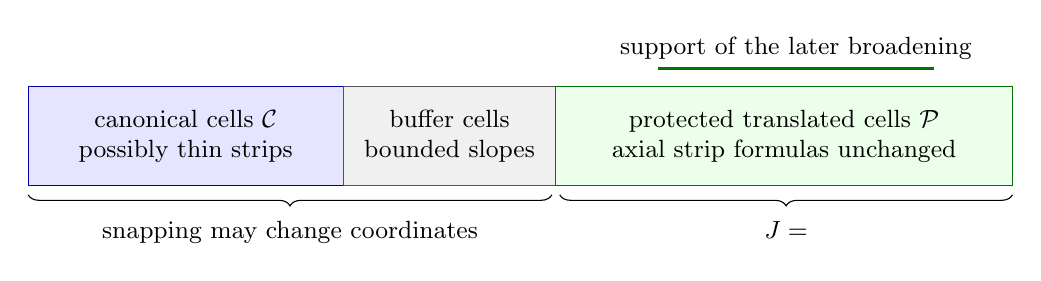
\begin{tikzpicture}[x=1cm,y=1cm,font=\small]
\filldraw[fill=blue!10,draw=blue!65!black] (0,0) rectangle (4,1.25);
\filldraw[fill=gray!12,draw=gray!65!black] (4,0) rectangle (6.7,1.25);
\filldraw[fill=green!8,draw=green!45!black] (6.7,0) rectangle (12.5,1.25);
\node[align=center,text width=3.7cm] at (2,.625)
  {canonical cells $\mathcal C$\\possibly thin strips};
\node[align=center,text width=2.4cm] at (5.35,.625)
  {buffer cells\\bounded slopes};
\node[align=center,text width=5.5cm] at (9.6,.625)
  {protected translated cells $\mathcal P$\\axial strip formulas unchanged};
\draw[decorate,decoration={brace,mirror,amplitude=4pt}]
  (0,-.12) -- (6.65,-.12)
  node[midway,below=6pt,align=center] {snapping may change coordinates};
\draw[decorate,decoration={brace,mirror,amplitude=4pt}]
  (6.75,-.12) -- (12.5,-.12)
  node[midway,below=6pt] {$J=\Id$};
\draw[very thick,green!45!black] (8,1.48) -- (11.5,1.48);
\node[above,align=center] at (9.75,1.48)
  {support of the later broadening};
\end{tikzpicture}
\caption{A schematic local passage from canonical cells to an interior
protected region.  The buffer already has quantitative parameter bounds,
so only the forward Lipschitz bound for its snapping map is needed.
Snapping fixes the protected region; broadening is supported strictly
inside it.  The bands depict adjacency, not metric widths or the global
topology of the subcomplexes.  Protected cells at the outer patch boundary
instead lie in the quantitative clustered belt.}
\label{ms:fig-protected-buffers}
\end{figure}

\subsection{Broadening the protected strips}

\begin{lemma}[Simultaneous broadening by an ambient flow]
\label{ms:broadening}
On the deep protected translation regions of
Lemma~\ref{ms:translations}, after snapping, the half-width can be
increased from $a_0=c_0W$ to
\begin{equation}
 a_1=(1-C\eta)W/2,
 \label{ms:wide-halfwidth}
\end{equation}
with fixed slack below half the regular slab gap.  It equals $a_1$
outside larger excluded-set buffers and equals $a_0$ near the edge
of the protected region.  The change is induced by a common
ambient locally bi-Lipschitz homeomorphism preserving every layer
parameter.  The resulting pre-slope density is bounded by
$CM_\sigma$ throughout the sharp construction.  On a region of
constant width $a_1$,
\begin{equation}
 \nabla u_j=\epsilon_j e_i+O(\eta),\qquad
 |\nabla u_j|\le1+C\eta,
 \qquad \epsilon_j\in\{-1,1\},
 \label{ms:sharp-scalar}
\end{equation}
where the error is in aligned coordinates and may be made smaller
than any prescribed multiple of $\eta$ except for the fixed
slot-loss contribution in the principal component.
\end{lemma}

\begin{proof}
Choose a common smooth cutoff supported well inside the unchanged
translation subcomplexes, equal to one beyond larger excluded-set
buffers.  Mollified distance cutoffs give derivative
$O(1/(NW))$ when the buffer width is $NW$.  First take the fixed
integer $N$ sufficiently large, depending on the slot margins and
the previously fixed constants.  Let $a(x)$ vary between $a_0$
and $a_1$ using this cutoff, so $|\nabla a|\le C/N$.

On a supporting main triangle $P$, let $l_P(x)$ be signed axial
height above its plane, with sign chosen according to increasing
layer parameter.  Use the strip $|l_P|\le a(x)$ and the layer
parameter given by affine conversion of $l_P/a$:
\begin{equation}
 u_P(x)=\frac W2\left(1+\frac{l_P(x)}{a(x)}\right).
 \label{ms:wide-parameter}
\end{equation}
The support of the change is far enough from the main triangle
boundary, from all unswitched fine triangles, and from all
non-slab, crease, face, and nonregular exclusions that every
supporting-plane formula required within several multiples of
$W$ is valid.  Same-family gaps from Lemma~\ref{ms:slots}, including
the opposite parallel band, stay larger than the two half-widths
with fixed slack.  The slice slopes are small because the
supporting planes are near horizontal and $|\nabla a|$ is small.
In independent mode the only possible concurrent strips have
near-independent coordinate normals.  These facts remain true
on a small open enlargement of each interval
$l_P/a\in[-1,1]$.

We verify that this simultaneous change preserves the parameter
topology.  Interpolate smoothly in time from $a_0$ to $a(x)$,
writing $a_\tau(x)$, $0\le\tau\le1$, with the same spatial
cutoff.  On each relevant plane neighborhood impose
\begin{equation}
 D_x(l_P/a_\tau)X_\tau
       +\partial_\tau(l_P/a_\tau)=0.
 \label{ms:material}
\end{equation}
Locally the list of possible constraints contains one member or
an independent pair.  Their gradients have the same independence
as the near-axis normals, since
\[
 D_x(l_P/a_\tau)
   =a_\tau^{-1}
       \left(\nabla l_P-(l_P/a_\tau)\nabla a_\tau\right).
\]
Thus the linear equations have a smooth local solution.  For
example use the right inverse of the one-row or two-row gradient
matrix.  The right sides are linear in $\partial_\tau a_\tau$,
and this choice has size $O(W)$ on the necessary open strip
neighborhoods.  Take a finite space-time cover such that every
neighborhood's list includes all constraints potentially present
there.  A smooth partition of unity preserves the linear
equations on their required sets.  Include the complementary
region with zero field, and arrange zero wherever
$\partial_\tau a_\tau=0$; the local choices are linear in that
quantity.  The field is compactly supported in the finite patch.

Its flow exists on the whole time interval.  Increase the buffer
factor if necessary so its $O(W)$ motion stays within all the
supporting-plane and endpoint extension margins.  Equation
\eqref{ms:material} makes $l_P/a_\tau$ constant along the flow.
The backward flow gives the converse, so all strip boundaries and
all layer parameters are transported exactly.  In particular this
is a common ambient change of both systems.  It leaves the
nonflat seams unchanged and preserves the joint product
trivializations and the PL-in-changed-coordinates property.
No uniform derivative bound for the flow or its inverse is needed.

The quantitative bound is obtained directly from
\eqref{ms:wide-parameter}, not by differentiating that flow:
\[
 \nabla u_P
   =\frac W{2a}\left(\nabla l_P-(l_P/a)\nabla a\right).
\]
Since $a\ge c_0W$, $|l_P|\le a$, and the plane slopes and
$|\nabla a|$ are bounded, this is bounded by a fixed constant.
Broadening occurs only on low-leakage tetrahedra, where
$s_\sigma$ is comparable to $W$.  Elsewhere the snapped bound is
$CM_\sigma$.  Thus this bound holds everywhere.  When $a=a_1$,
$\nabla a=0$, $\nabla l_P=\epsilon_je_i+O_\eta(\delta')$, and
$W/(2a_1)=1+O(\eta)$.  Taking the remaining tolerances as in
Lemma~\ref{ms:slots} proves \eqref{ms:sharp-scalar}.
\end{proof}

\begin{proposition}[Sharp-island geometric contract]
\label{ms:sharp-contract}
Fix $\eta$, the compact chart and basis bounds, and the finite
template choices above.  The calibrated islands admit pre-stacks
with all the qualitative properties of Definition~\ref{wl:prestack} and
with the following quantitative properties.
\begin{enumerate}
\item Throughout an enlarged equal-weight island the pre-slope
density is at most $CM_\sigma$ in aligned units.  This constant
is independent of microscopic master widths, central crossing
angles, final guard gaps, $H$, $W$, and the final level-count
tolerance $\delta'$.
\item In deep regular low-leakage portions, the scalar gradients
obey \eqref{ms:sharp-scalar}.  At concurrent independent strips
the two-coordinate squared Frobenius cost is at most $2+C\eta$.
At an occupied diagonal transition after routing, the active
coordinate has gradient $\pm\nabla u_j\pm\nabla u_k$, whose
squared norm has the same bound.  In parallel mode the opponent
bands are disjoint in these portions and the squared norm is at
most $1+C\eta$.  Occupied-stair speeds multiply these bounds by
at most $(1+C\zeta)^2$.
\item In a regular tetrahedron the excluded $CNW$ neighborhoods
of its faces, all its main slab creases, and its non-slab disks
occupy relative volume at most
\begin{equation}
 C_N\left(\frac WH+\delta'\right).
 \label{ms:dirty-volume}
\end{equation}
The canonical protection and broadening margins only change the
fixed factor $C_N$.  Nonregular tetrahedra, high-leakage
tetrahedra, their required fixed-neighbor layers, and patch
boundary margins are charged by their full $M^p$-cost.
\end{enumerate}
The norm statements concern the smooth compatible label sectors
after the combined label barrier, away from central radial
activation cutoffs.  They are geometric scalar-pair estimates;
their physical conversion and the saturation argument are made
in Lemma~\ref{ha:saturation}.
\end{proposition}

\begin{proof}
The master construction, the translation switch, the canonical
snapping, and the common broadening flow preserve the entire
two-colour pattern and its parameters, as proved above.  In the
canonical region all displacements are at most $Cs_\sigma$.
In particular the larger translation displacement $a_0$ is used
only when $s_\sigma$ is comparable to $W$.  Thus
Lemma~\ref{ms:bounded-complexity} applies there, and
Lemma~\ref{ms:snapping} gives the first assertion in the formerly
uncontrolled region.  Its buffer cells use only a uniform upper
Lipschitz bound for the map from new to old coordinates and an
already quantitative master bound.  Ordinary weak widths may
be larger outside the canonical region, but their transition is
fully clustered and has the same $CM_\sigma$ bound in the
equal-weight belt, or the ordinary edge bound outside it.
Finally Lemma~\ref{ms:broadening} supplies the remaining transition and
deep-strip estimates.  The finite representatives, slot margins,
and chart factors were all fixed before the small count errors,
so no new dependence on those errors has entered.

In independent mode the two indicated axes are orthogonal.
Equation \eqref{ms:sharp-scalar} gives squared Frobenius norm at
most $2+C\eta$ when both coordinates contribute.  A routed
diagonal has parameter $d=w_j-u_j+u_k$, with possible
coorientation changes.  Hence its gradient is the asserted
signed sum of two near-orthogonal covectors, with the same bound.
Only one output coordinate is active on that transition.  In
parallel mode the two bands are separated by the axial gap, so
they have no such overlap in the protected region.  The
occupied-interval stair conversion has speed at most
$1+C\zeta$, giving the stated factor.  These statements use the
combined label pinning to identify the intended smooth sector;
they assert no estimate across an unrelated sector or an active
central cutoff.

For the volume estimate, there are $O(H/W)$ slab disks, each
with at most one main crease of length $O(H)$.  Their
$CNW$-tubes cost at most $C_NH^2W$.  There are at most
$C\delta'H/W$ non-slabs, each of area $O(H^2)$; thickening
their finitely many main triangles by $CNW$ costs at most
$C_N\delta'H^3$ (the smaller edge and vertex terms are absorbed
when $W/H$ is small).  The tetrahedron-face buffers cost
$C_NH^2W$.  Divide by volume comparable to $H^3$ to obtain
\eqref{ms:dirty-volume}.  Auxiliary cells have size at most
$CW$, so trimming protected subcomplexes and reserving the
flow neighborhoods only enlarge this fixed buffer factor.
For nonregular and high-leakage sets use
Lemma~\ref{ms:majorant}; the appropriate analytic error tests in
Lemma~\ref{ha:sharp-counts} make their full costs small.  No small
volume assertion for those uncontrolled tetrahedra is being
used in place of that $M^p$ payment.
\end{proof}

\subsection{The pre-stack contract and the order of constants}

\begin{proposition}[Geometric realization of pre-stacks]
\label{ms:prestacks}
Suppose the central starting systems have the boundary data of
Lemma~\ref{ms:boundary-collar} and the wall-by-wall edge upper counts
used in the separate-colour normalization of
Proposition~\ref{wl:normalization}.  Suppose also that the weighted edge tests
have been selected as in Lemma~\ref{ms:edge-tests}.  The constructions
of Sections~\ref{sec:mesh} and~\ref{sec:calibrated-islands} give the
pre-stacks required in
Definition~\ref{wl:prestack}: same-colour compact disjoint collars; opposite
arc or circle products with the full parameter rectangles;
individual pattern trivializations preserving the opposite
parameter; the exact boundary correspondence; and locally
bi-Lipschitz changed coordinates in which the relevant endpoint
arrangements and parameters are PL.

Their pre-parameter slopes admit a density $G$ satisfying the
ordinary bound \eqref{ms:weak-G}, the fixed boundary and chart
bounds of Lemma~\ref{ms:boundary-collar}, and the island bound
$G\le CM_\sigma$ of Proposition~\ref{ms:sharp-contract}.  All constants in
these inequalities may be fixed before choosing final guard
gaps, mesh resolutions, and sample weights.  Consequently any
crude compact-local integral capacities deduced from these
inequalities and the conditional edge-variation bounds are
independent of those later choices.  The actual simultaneous
choice of the capacities, meshes, and samples is supplied by
Lemma~\ref{ha:capacities} and Proposition~\ref{ha:initial-walls}.
\end{proposition}

\begin{proof}
Normalize one colour at a time, keeping its specified boundary
traces and without increasing any individual wall--edge count.  For this
conclusion only the resulting normal data
are needed; an ambient normalization isotopy need not fix the
other colour.  The weak templates give the claimed collar and
pattern properties away from the calibrated islands.  On the
islands the master construction has the same properties and
the subsequent common ambient changes preserve them exactly.
All attachments to the outer collar use its joint trivialization.
In particular no step merely chooses independent individual
product charts and assumes they preserve the other coordinate.
Compactness of each individual sampled wall and local
finiteness of the family give the required qualitative local
bi-Lipschitz statements for each fixed construction.

We make the constant order explicit.  First fix coarse working
charts, compact basis bounds, feature lengths and aspect bounds,
the slot loss $\eta$, and the weak boundary-jitter slack.  Fix
the resulting finite weak template list, its angle tolerances,
and the boundary compression $\varepsilon$.  These fix the
normal-template shapes, the auxiliary neighbor-ratio bounds,
the cardinality of the canonical arrangements, all finite
representatives in Lemma~\ref{ms:snapping}, and the translation and
broadening buffer factors.  On a given compact their constants
are finite, though they need not be small.  Next choose the
level-edge tolerance and generic perturbation fractions small
against those fixed bounds; in calibrated patches fix also the
chart and ambient-jitter error fractions.  Their possibly large
density constants are then known.  The analytic mean errors
are chosen smaller afterward.  None of these choices involves
the eventual guard gaps.

Fix the local edge-variation and density bounds, including any
chart weights, before the guard nets are set.  They give finite
candidate capacities for $\int G^p$ by
\eqref{ms:weak-G}, \eqref{ms:majorant-power}, and the fixed
boundary terms.  Having chosen the guards and their forbidden
label neighborhoods, take $d_0$, the mesh, and every displacement
fine enough for the associated spatial buffers.  Boundary warp
motion has size $O(\delta)$ with $\delta\ll d_0$; its inverse
label constants do not deteriorate under this thinning.  The
interior meshes keep their shape lists under refinement and
their fixed jitter density factors.  Sample last, taking all
feature slots sufficiently fine and, in the finitely many
equal-weight islands, $W/H$ as small as necessary.  Arbitrarily
small allowed feature components do not obstruct this final
refinement.  Whole-interval and occupied-interval stair errors
charge absolute gap lengths and rounding errors, so they may
also honor the already prescribed guard and label accuracies.

Microscopic master widths introduce no additional capacity
constant.  They are removed precisely on the canonical cells
by a map with uniformly bounded upper Lipschitz constant, while
the direct representative-label estimate is $CW/s_\sigma$.
Subdivision uses displacement differences and introduces no
$H/W$ loss.  The final broadening estimate comes directly
from \eqref{ms:wide-parameter}.  The qualitative inverse bounds
of the common coordinate changes, the pattern trivializations,
and the eventual product or ball extensions in
Theorem~\ref{wl:realization} are never substituted into these estimates.

For path estimates take upper slopes relative to the closed
parameter domains, as defined in Lemma~\ref{ms:snapping}, with
adjacent-cell maxima.  The fixed-input parameters are locally
Lipschitz on their compact collars.  On exceptional
lower-dimensional interface strata one may enlarge $G$ further
to any necessary actual local collar Lipschitz bound, with
locally finite prescriptions.  Such strata have zero ambient
volume.  This gives the pointwise control needed for
one-dimensional coarea on restricted path portions without
asserting a uniform two-point Lipschitz bound across arbitrary
gaps between parameter pieces.  It changes none of the stated
integral capacities.
\end{proof}
